%!TEX root = ../thesis.tex

\ifpdf
    \graphicspath{{ChapterDAQ/Figs/Raster/}{ChapterDAQ/Figs/PDF/}{ChapterDAQ/Figs/}}
\else
    \graphicspath{{ChapterDAQ/Figs/Vector/}{ChapterDAQ/Figs/}}
\fi

% ******************************* DAQ schema ****************************
\chapter{Data Acquisition Architecture}

\nomenclature[z-SCT]{SCT}{SemiConductor Tracker}
\nomenclature[z-L1A]{L1A}{Level 1 Accept}
\nomenclature[z-DCS]{DCS}{Detector Control System}
\nomenclature[z-BST]{BST}{Beam Synchronous Timing system}


My work focused on the understanding of the Trigger and Data Acquisition System (DAQ), as well as, implement the controls for the Trigger Logic Board (TLB) that is at the center of Fig.\ref{fig:DAQArchitecture} and a core component of the data taking. I will first, however, describe the general layout of the data acquisition so that the reader has a better understanding of the TLB's role in FASER.

The DAQ architecture digests information from three different kinds of detectors (in grey in Fig. \ref{fig:DAQArchitecture}), 72 SemiConductor Tracker modules (SCT), 10 scintillators and 4 calorimeters. The SCT modules are connected to tracker readout boards whereas the scintillators and calorimeter are connected to the digitizer. The signals from the scintillators and calorimeters are combined in pairs (AND, OR or one-only) to form 8 trigger outputs that go straight into the TLB. The TLB then maps the 8 trigger outputs into 4 final trigger lines via a Look-up Table described in section \ref{LUT}. Any signal in the 4 trigger lines will ultimately decide whether we want to save the signal as a physical event or not. The tracker modules do not contribute to forming a trigger decision, this is done solely using calorimeter and scintillator information. They are readout on a trigger accept signal only. On top of the four trigger lines coming from the scintillators and the calorimeters, two additional trigger accept signals can be created by a random trigger or software trigger generated internally by the TLB. In total, the TLB outputs six trigger lines, that can all be prescaled or vetoed, and form a Level 1 Accept (L1A). If the board decides to save the event for further analysis, it sends the L1A signal to both the digitizer and to the tracker readout boards which initiates the read-out of the subdetector's event data from the respective onboard buffers to the data acquisition server in a server room above ground.

Additionally, the TLB needs to receive time information through the LHC beam synchronous timing system (BST). The orbit can be passed directly via LEMO cable to the TLB. This information is then used to assign the Bunch Crossing Reset (BCR) signal. The clock signal however needs to pass through a "clock cleaner" which is a commercial board that ensures stables and high quality clock signal.

\begin{figure}[htbp!] 
\centering    
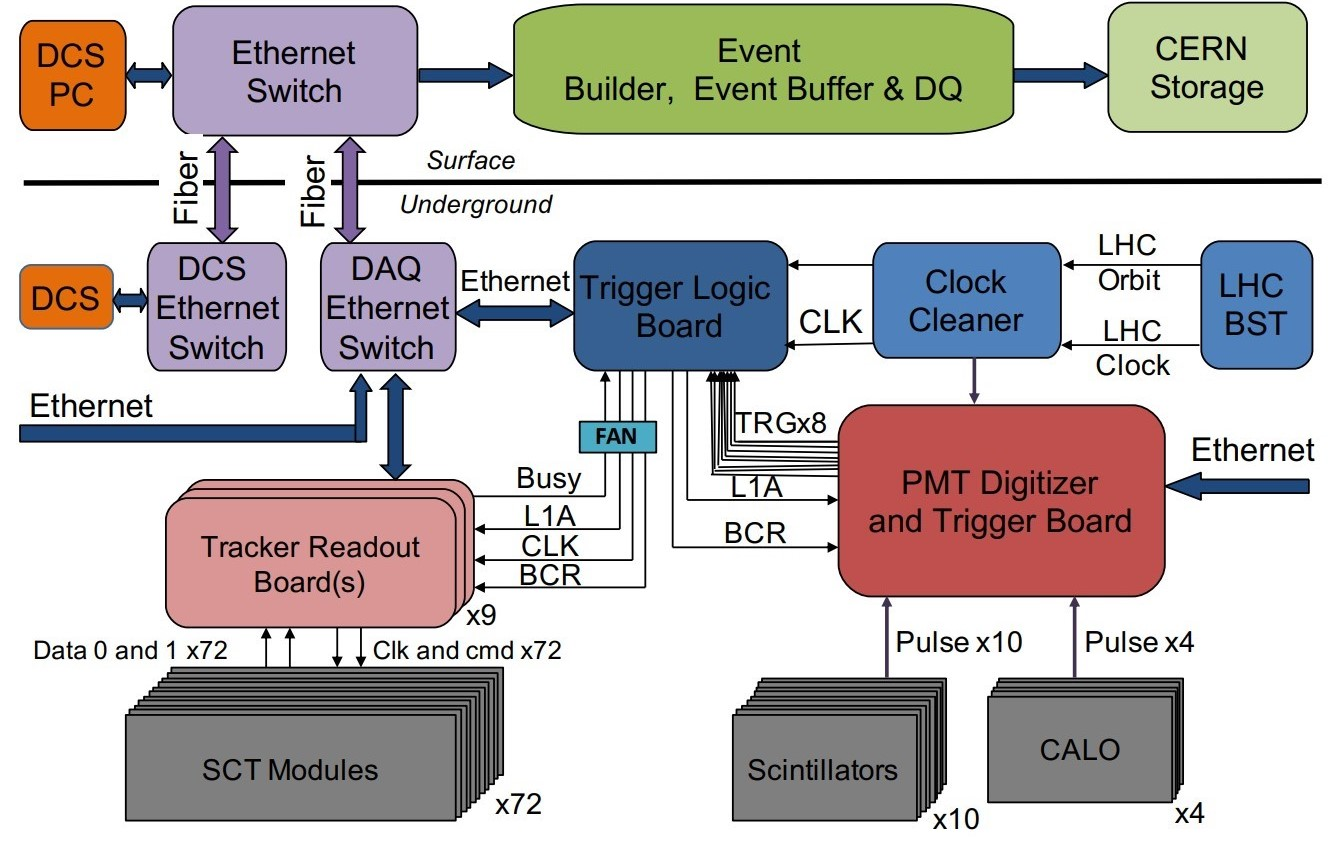
\includegraphics[width=0.8\textwidth]{ChapterDAQ/Figs/GeneralDAQ/Architecture.jpg}
\caption[DAQ Architecture]{DAQ Architecture - The TLB processes trigger signals from the scintillators and the calorimeter and returns an L1A to the tracker board and the digitizer.}
\label{fig:DAQArchitecture}
\end{figure}


\section{DAQ Dataflow}

\nomenclature[z-ECR]{ECR}{Event Counter Reset}
\nomenclature[z-RO]{RO}{Read-Out}
\nomenclature[z-ROR]{ROR}{Read-Out Receiver}
\nomenclature[z-EB]{EB}{Event Builder}

\begin{figure}[htbp!] 
\centering    
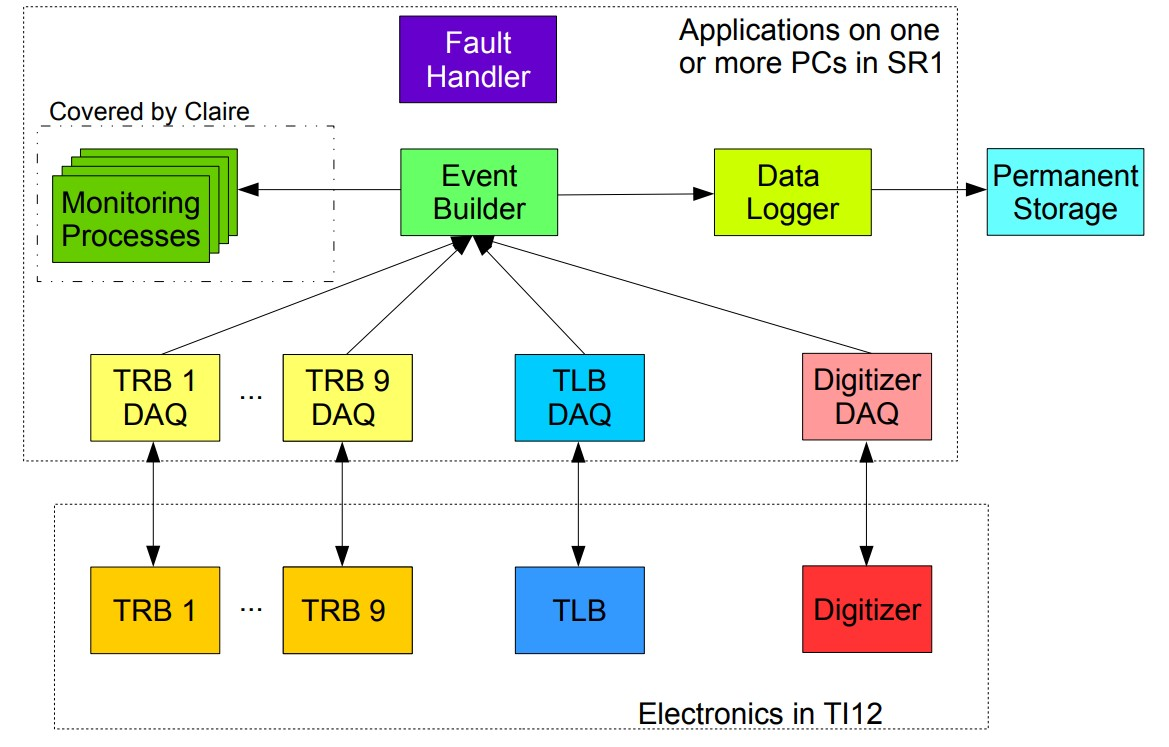
\includegraphics[width=0.8\textwidth]{ChapterDAQ/Figs/GeneralDAQ/DAQDataFlow.jpg}
\caption[DAQ Dataflow]{DAQ Dataflow - The front-end electronics will each have their own receiver application which takes the initial raw data, adds a fragment header and sends it to the Event Builder.}
\label{fig:DAQDataFlow}
\end{figure}

Once an L1A has been sent out to all detectors, the event's data acquisition can start. It takes place in three different stages - combining more and more the different detectors data into a single event, see Fig.\ref{fig:DAQDataFlow}.

Each front-end electronics board located in TI12 (TRB, TLB, Digitizer) will have its own "receiver" application which will take the inital raw data from the read-out boards (ROs) whenever it receives a trigger. These receiver applications are board-specific because they need to send and check board configuration before each run. They will also be able to send special commands to the electronics during runs such as the ECR (Event Counter Reset). Moreover, each read-out receiver application (RORs) will take the raw data payload and add a  "fragment header" that contains important summary information of the event such as Event ID, BCID and size of the payload to form "fragments", see Table \ref{table:RORHeader}. The Event ID (number of triggers received since start) and BCID (bunch crossing ID) are embedded information in the raw payload that is extracted to construct the fragments.

After that, each receiver application sends out its data fragments to a single Event Builder (EB) application that will merge all fragments with the same event ID into a single event with an additional "event header". The event builder can check at this moment if no error is present by cross checking between each fragments if the BCID match.



\begin{table}[htbp!] 
\caption{ROR event header assigned by the receiver applications}
\centering
\label{table:RORHeader}
\begin{tabular}{c c}
\toprule
ROR event header & Size (bits) \\
\midrule
Start of header marker & 8\\
Fragment tag & 8\\
Trigger bits & 16\\
Format version number & 16\\
Total header size & 16\\
Total data size & 16\\
Source identifier & 32\\
Event ID & 64\\
Bunch crossing ID & 16\\
Data status & 16\\
Time-stamp & 64\\
\midrule
Total size & 288 (9 4-byte words)\\
\bottomrule
\end{tabular}
\end{table}

\begin{table}[htbp!] 
\caption{Full event header assigned by the EB}
\centering
\label{table:FullEventHeader}
\begin{tabular}{c c}
\toprule
Full event header & Size (bits) \\
\midrule
Start of header marker & 8\\
Event tag & 8\\
Trigger bits & 16\\
Format version number & 16\\
Total header size & 16\\
Total data size & 16\\
Number of fragments & 8\\
Run number & 24\\
Event ID & 64\\
Event Counter & 64\\
Bunch crossing ID & 16\\
Data status & 16\\
Time-stamp & 64\\
\midrule
Total size & 352 (11 4-byte words)\\
\bottomrule
\end{tabular}
\end{table}

A small note on why the ECR is needed: the electronic boards only use 24-bit counters which are filled in $\sim7$ h at the maximum expected rate of 650 Hz that we need to reset as we want to run for longer periods. This is why the Event ID in the ROR and EB is 64 bits, ensuring each event has a unique 64-bit event ID even though the event counter is periodically reset. The first bits will be used to count the number of ECR.

\section{Run Control}

During FASER runs, everything will be launched, controlled and configured using the web-based run-control application, see Fig. \ref{fig:RunControl}. It will feature basic DAQ control commands such as initialise, start, ECR, stop and shutdown. Additionally, a configuration window will quickly let the user change the configuration json (details: \ref{configuration}) and a run information panel will help visually monitor the physics and monitoring rate. Finally, a status and settings panel will indicate whether each module (trigger, eventbuilder, datalogger, etc.) is running or stopped and let the user easily access the logs.

\begin{figure}[htbp!] 
\centering    
\frame{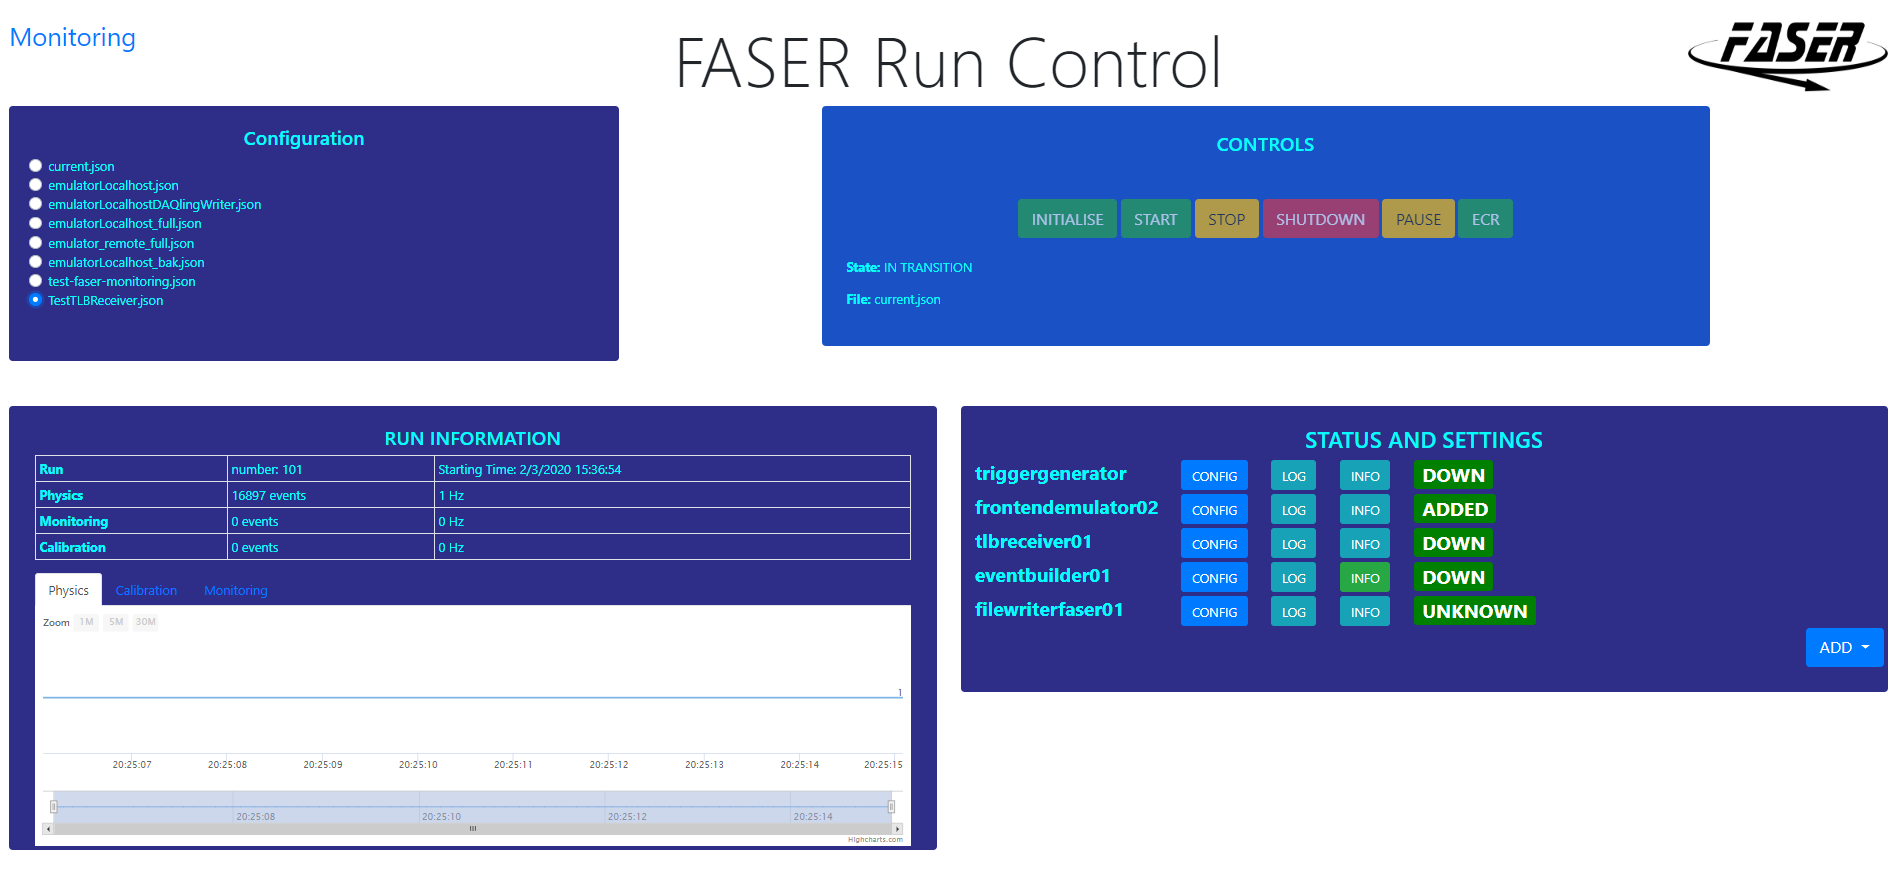
\includegraphics[width=0.8\textwidth]{ChapterDAQ/Figs/GeneralDAQ/RunControl.png}}
\caption[DAQ Run Control]{DAQ Run Control - This run control allows to interface with the experiment during data taking. It is accessed on a browser and used to set configurations on the different detectors and start/stop the DAQ. It can also display live data from the experiment using metrics.}
\label{fig:RunControl}
\end{figure}

\subsection{Displaying Data using Grafana}

Monitoring will be done using Grafana \cite{noauthor_grafana_nodate}, a multi-platform open source analytics and interactive visualization software. This will let the user do basic statistics such as average and rate of physics event. The implementation in the different modules, see section \ref{TriggerReceiverModule}, is done by adding a metric to the selected variable chosen to be visualized in the code. For example, one would simply declare the metric
\begin{lstlisting}
std::atomic<int> my_ metric1;
\end{lstlisting}
and then increment it whenever a physics event has been detected.
\begin{lstlisting}
my_metric1 +=1;
\end{lstlisting}
The metric is periodically registered in a monitoring database which Grafana interfaces with. The monitoring database used is Influxdb \cite{noauthor_influxdb_nodate} - an open-source time series database.

\begin{figure}[htbp!] 
\centering    
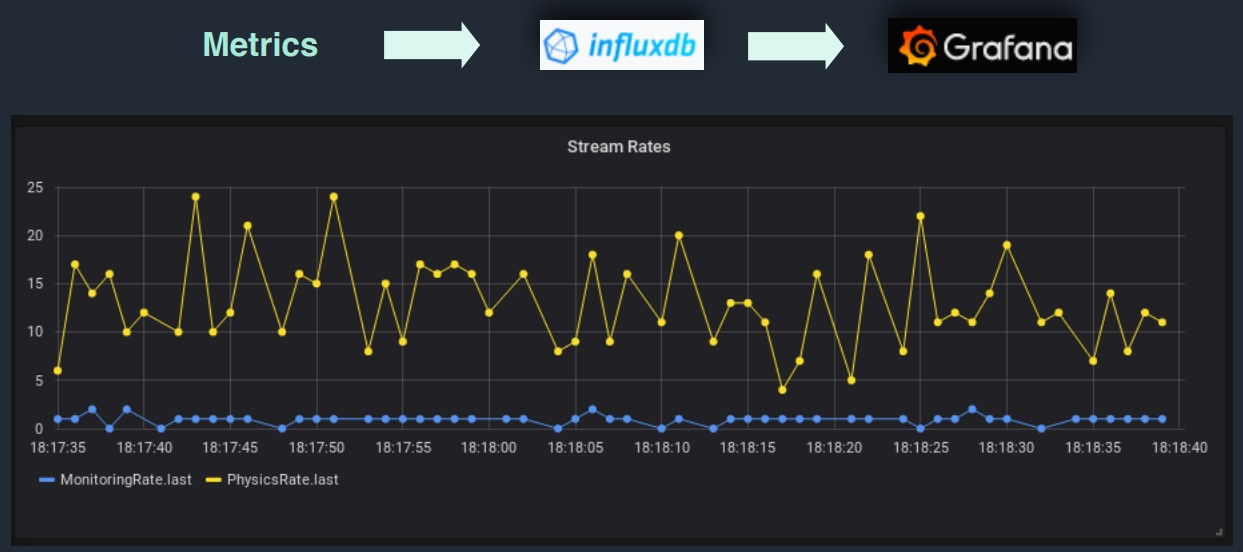
\includegraphics[width=0.8\textwidth]{ChapterDAQ/Figs/GeneralDAQ/Grafana.jpg}
\caption[Grafana]{The metric variable would be processed by Influxdb and then by Grafana to produces visualisations graphs.}
\label{fig:Grafana}
\end{figure}


% ******************************* Trigger and Data Acquisition ****************************
\chapter{Trigger and Data Acquisition}
\section{Unige USB3 GPIO}

\begin{wrapfigure}{R}{0.38\textwidth}
\centering    
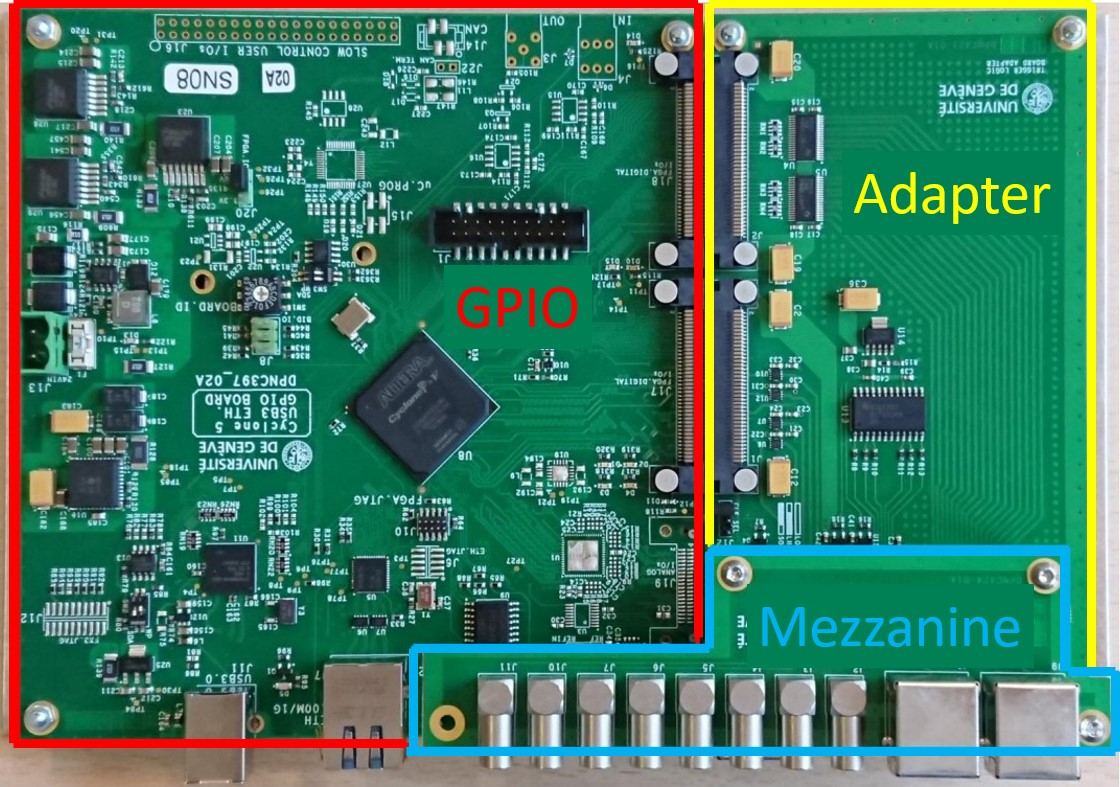
\includegraphics[width=0.36\textwidth]{ChapterDAQ/Figs/GeneralDAQ/UnigeUSB3GPIO.jpg}
\caption[Unige USB3 GPIO]{The TLB uses the same Unige USB3 GPIO board as the TRB for the "core", highlighted in red. An additional adapter board and mezzanine are used to interface with hardware signals.}
\label{fig:UnigeUSB3GPIO}
\end{wrapfigure}

The Trigger Logic Board (TLB) and the Tracker Readout Boards (TRB) are both designed to be the interface between the hardware signals and the readout and control. The TRB digest signals straight from the SCT modules whereas the TLB receives the scintillators and calorimeter signals through the Digitizer. The solution is to use a GPIO (General Purpose Input-Output) developed by the University of Geneva called the "Unige USB3 GPIO" for both the TLB and the TRB as core module \footnote{The core of the board is an Intel Cyclone V A7 FPGA} with an additional dedicated interface board for each application, see Fig. \ref{fig:UnigeUSB3GPIO}. For the readout and the slow control, two interfaces can be used: USB3 and Ethernet. USB3 has initially been used but ultimately Ethernet will be the means of communication \cite{faser_collaboration_technical_2018}.


Both TLB and TRB boards have a standalone GUI to perform the initial testing. As an example, Fig. \ref{fig:DAQGui} shows the TLB's GUI and its three tabs. The "board" tab controls the DAQ start and stop as well as sending direct parameters through slow control such as enabling or disabling the trigger and sending software triggers. The second tab is used to toggle the eight inputs that come in through the LVDS. It also allows the prescales to be set and additional control such as enabling the LHC Clock or using the on-board one.  The last tab is a 256 entries matrix that allows to set the LUT (more information in \ref{LUT}).

\begin{figure}[htbp!] 
\centering    
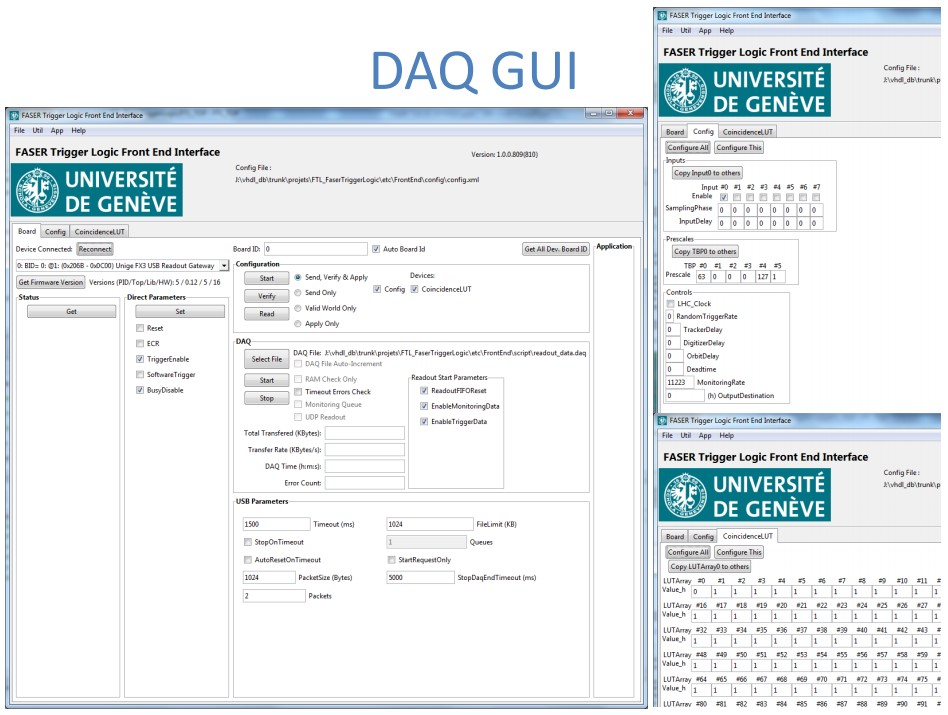
\includegraphics[width=0.8\textwidth]{ChapterDAQ/Figs/GeneralDAQ/DAQGui.jpg}
\caption[DAQ GUI]{The DAQ GUI has three tabs, one to start DAQ and send slow control commands, one to configure inputs and prescales and the last one to set the LUT.}
\label{fig:DAQGui}
\end{figure}

Once the data acquisition is started, the TLB can output two types of data: trigger data or monitoring data depending on which one was enabled. The trigger data is sent out in chunks  of 5 "words" of 32 bits, see Fig. \ref{fig:ReadoutData}.

First a header is used to mark the beginning of the incoming trigger data. The second word contains the Event Counter coded into 24 bits and the third word uses the whole 32 bits to code the orbit counter. The fourth word is the Bunch Counter (0 to 3563) that uses the required 12 bits. The fifth and last word code different information. The first bits code the Input bits (next clock) and Input Bits. Bits 16 to 21 code the Trigger Before Prescale (TBP) where each of the bits is a trigger signal. Bits 24 to 29 code the Trigger After Prescale (TAP).

The Monitoring Data, used for debugging, follows the same word order but has a total of 25 words to code more information. Because the Monitoring Data rate is low compared to the Trigger Data\footnote{Max trigger rate: 1 kHz, Monitoring rate: 0.001 Hz to 11.2 kHz}, several triggers will arrive in between monitoring data as well as information on events that are vetoed and thus not recorded as Trigger Data. This is why TBP now uses whole words to count up the hundreds or thousands of trigger that will have arrived and are now labelled TBP0 to TBP5. Additional Trigger after veto are used to count the trigger that have been vetoed and finally, the last four word code the different sources of veto. The full TLB data format is showed on Fig. \ref{fig:TLBDataFormatPDF}.


\begin{figure}[htbp!]
   \centering
    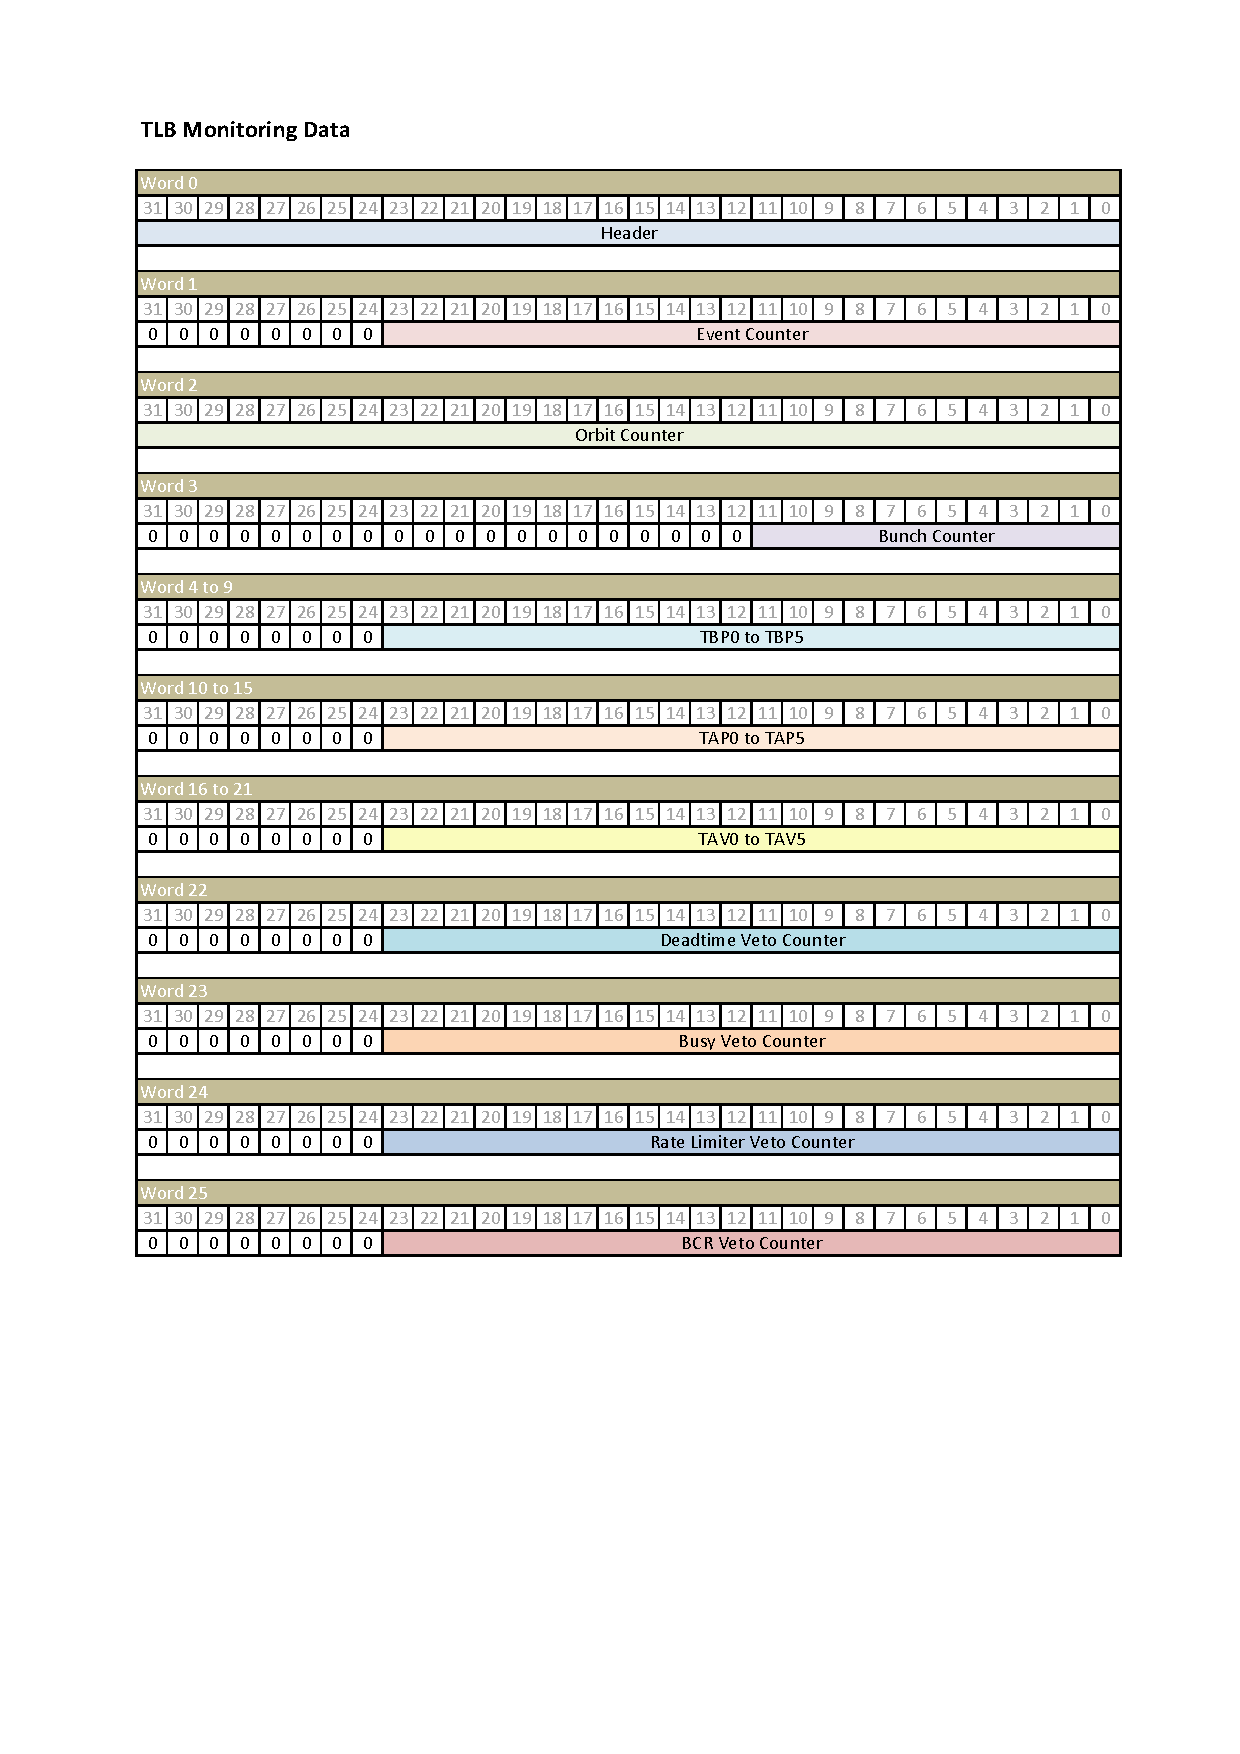
\includegraphics[page=1,width=.8\textwidth, trim={2.0cm 8.0cm 1.7cm 1.8cm}, clip]{Appendix3/TLBdataformat.pdf}
   \includegraphics[page=2,width=.8\textwidth, trim={2.0cm 18.5cm 1.7cm 1.8cm}, clip]{Appendix3/TLBdataformat.pdf}
 \caption{TLB Data Format}
 \label{fig:TLBDataFormatPDF}
\end{figure}



\begin{figure}[htbp!] 
\centering    
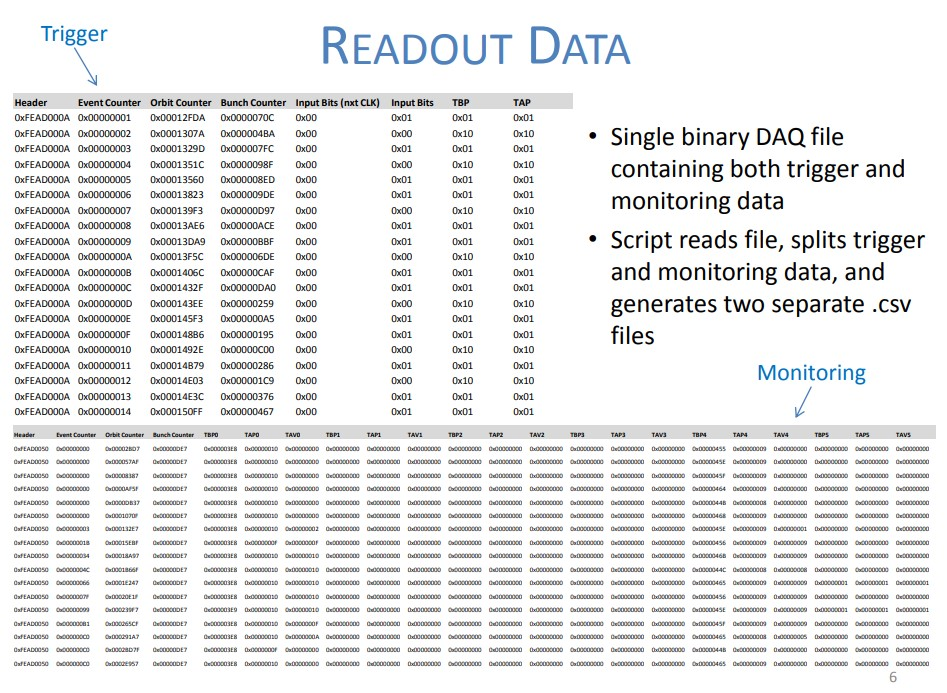
\includegraphics[width=0.8\textwidth]{ChapterDAQ/Figs/GeneralDAQ/ReadoutData.jpg}
\caption[TLB Trigger and Monitoring Data output]{The TLB can output Trigger Data and/or  Monitoring Data.}
\label{fig:ReadoutData}
\end{figure}


% ******************************* TLB Board ****************************
\section{TLB Board}

\nomenclature[z-SC]{SC}{Slow Control}
\nomenclature[z-BCR]{BCR}{Bunch Crossing Reset}

The TLB is the central triggering module of the FASER TDAQ system. It
receives input signals at 125 MHz from the scintillators and the calorimeter that have been converted into computer-readable information via the digitizer\footnote{The digitizer, a CAEN VX1730 VME board, samples at 500 MHz, but its coincidence logic and outputs run at 125 MHz.}. The TLB processes these signals to create the trigger decision (L1A) which is sent to the detector readout boards. The TLB is the brain of FASER as it receives signals from every detector and then takes the decision to store the event or not. A flow chart presenting the operation of the TLB is shown on Fig.\ref{fig:TLBSchema}. The eight signals from the digitizer come in the TLB in the bottom right corner of the figure \ref{fig:TLBSchema}. These eight trigger lines coming from the CAEN digitizer are synchronized to the 40 MHz clock which can be selected to either come from an on-board clock or - during operations - from the LHC clock. The LHC clock signal is processed by a clock cleaner board before coming in the TLB. Each of the eight channels can then be individually delayed to account for differences in cable length and then go into the coincidence logic detailed in subsection \ref{LUT} \nameref{LUT}. These four outgoing trigger lines, as well as the random trigger (TBP5) and a software trigger (TBP6)  both controlled via SC (Slow Control), can now be individually prescaled. More information on these modules can be found in subsection \ref{Prescales} - \ref{Software Trigger}. The signal from these six signals is almost ready to become an L1A. However, FASER has different sources of deadtime, see Table \ref{table:DeadtimeSources}, where it is unable to read data. In fact, the TLB must first verify that a previous L1A wasn't sent out the previous 5-10 $\mu s$ as the detector need this time to readout the data. It must also check that the signal is not within a few clock cycles of a BCR.

\begin{table}[htbp!] 
\caption{Sources of deadtime.}
\centering
\label{table:DeadtimeSources}
\begin{tabular}{l p{10cm}}
\toprule
Simple Deadtime: & Number of 25ns clock cycles after a L1A
where a new L1A is vetoed.\\
BCR: & A dead time is issued if a BCR was sent in the last 6 CLKs, this CLK or the next two CLK
cycles.\\
Busy (tracker): & Designed not to allow a new L1A while the tracker is reading out an event.\\
Rate Limiter: & Introduces dead time after three L1As in 15 turns. Triggers are rejected and  the output rate is kept below 2.25 kHz.\\
\bottomrule
\end{tabular}
\end{table}

\begin{figure}[htbp!] 
\centering    
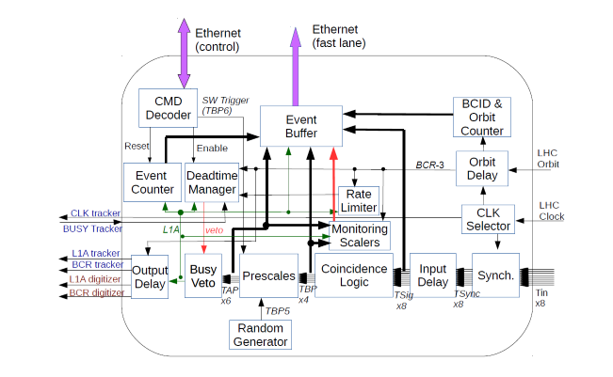
\includegraphics[width=0.7\textwidth]{TLBSchema.png}
\caption[TLB Schema]{TLB Schema - 8 trigger inputs are received from the right. Some coincidence logic is applied via a LUT and if no veto is applied it sends out an L1A to the tracker boards and the digitizer.}
\label{fig:TLBSchema}
\end{figure}

\section{LUT}
\label{LUT}

\nomenclature[z-LUT]{LUT}{Look Up Table}

\begin{wrapfigure}{R}{0.38\textwidth}
    \centering
    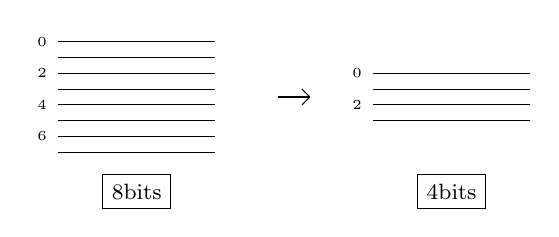
\begin{tikzpicture}
    %LUT
    \node[fill=white, text=black, draw=black] at (1,-0.5) {\footnotesize 8bits};
    \node[fill=white, text=black, draw=white] at (-0.2,1.4) {\tiny 0};
    \draw (0,0) -- (2,0);
    \draw (0,0.2) -- (2,0.2);
    \node[fill=white, text=black, draw=white] at (-0.2,1.0) {\tiny 2};
    \draw (0,0.4) -- (2,0.4);
    \draw (0,0.6) -- (2,0.6);
    \node[fill=white, text=black, draw=white] at (-0.2,0.6) {\tiny 4};
    \draw (0,0.8) -- (2,0.8);
    \draw (0,1.0) -- (2,1.0);
    \node[fill=white, text=black, draw=white] at (-0.2,0.2) {\tiny 6};
    \draw (0,1.2) -- (2,1.2);
    \draw (0,1.4) -- (2,1.4);
    
    \draw (2.8,0.7) -- (3.2,0.7);
    \draw (3.1,0.8) -- (3.2,0.7);
    \draw (3.1,0.6) -- (3.2,0.7);

    \node[fill=white, text=black, draw=black] at (5,-0.5) {\footnotesize 4bits};
    \node[fill=white, text=black, draw=white] at (3.8,1.0) {\tiny 0};
    \draw (4,0.4) -- (6,0.4);
    \draw (4,0.6) -- (6,0.6);
    \node[fill=white, text=black, draw=white] at (3.8,0.6) {\tiny 2};
    \draw (4,0.8) -- (6,0.8);
    \draw (4,1.0) -- (6,1.0);

    \end{tikzpicture}
    \caption[LUT 8 to 4 bit conversion]{The TLB's LUT receives 8 bits and converts it to 4 bits.}
    \label{fig:LUT}
\end{wrapfigure}

The coincidence logic is done using a Lookup Table (LUT). The LUT is a 256 input table (8 bits) where each input receives a value from 0-16 (4 bits). The benefits of a LUT are that it saves precious computing time and is easily reprogrammable via slow control because it is stored in RAM. It works by receiving the eight input channels (TSig1-8) from the digitizer and outputting a 4 bit value accordingly. This 4 bit value are 4 user defined coincidence trigger lines before prescale (TBP1-4). This allows to setup complicated logic via software as opposed to via hardware.

Figure \ref{fig:LUT} helps visualize how the LUT converts the eight signals from the digitizer to 4 coincidence lines. One important thing to note is that every 256 values from the LUT must be configured every time the TLB is powered on because, as mentioned before, the LUT is stored in RAM. Table \ref{table:LUTtable} represents how the user would fill a LUT that triggers on the first channel - by assigning LutArray \#1 to 1.

\begin{table}[htbp!] 
\caption{An example of LUT setup in software.}
\centering
\label{table:LUTtable}
\begin{tabular}{l c c c c c c}
\toprule
LUTArray & \#0 & \#1 & \#2 & \#3 & \#n & \#255 \\
\midrule
Value & 0 & 1 & 0  & 0 & ... & 0 \\
\bottomrule
\end{tabular}
\end{table}

A few other examples are presented in Fig.\ref{LUTexamples}. The first example in Fig.\ref{fig:LUT1} shows a Trigger Signal (TSig) from the digitizer in the first channel as visualized by the red line in the zeroth bit. In this example we want to attribute a certain coincidence logic to when we have the first channel firing (and only the first channel firing, no other signal). This can be done by setting LUT\#1 to 1 so that when you have a signal in channel0 then you get 1 as output. It's important not to get confused by the indices, LUT\#0 represent all 8 bits off or in our example all bits to black. Because the first line is red we need to assign a value to LUT\#1. In our second example in Fig. \ref{fig:LUT2} a signal is incoming in the second channel of the digitizer so we want to decide what LUT\#2's logic will be. Here we decided we want to fire all the coincidence trigger lines before prescale so all the 4 bits are red, i.e. set to 16. In the last example we'll present a coincidence. Let's say the digitizer receives signals in channel 1 and 2 but you only want an L1A when they are both coming in together, then you can set LUT\#1=0 and LUT\#2=0 so that you don't trigger on single event but you set LUT\#3 to 1 so that L1A's are only sent during a coincidence.

%Examples
\begin{figure}[htbp!] 
\begin{subfigure}{.45\textwidth}
    \centering
    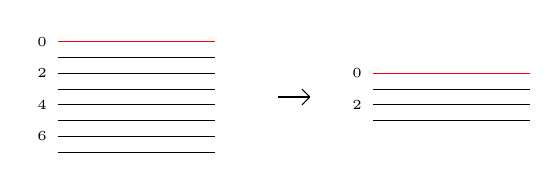
\begin{tikzpicture}
    %LUT
    \node[fill=white, text=black, draw=white] at (-0.2,1.4) {\tiny 0};
    \draw (0,0) -- (2,0);
    \draw (0,0.2) -- (2,0.2);
    \node[fill=white, text=black, draw=white] at (-0.2,1.0) {\tiny 2};
    \draw (0,0.4) -- (2,0.4);
    \draw (0,0.6) -- (2,0.6);
    \node[fill=white, text=black, draw=white] at (-0.2,0.6) {\tiny 4};
    \draw (0,0.8) -- (2,0.8);
    \draw (0,1.0) -- (2,1.0);
    \node[fill=white, text=black, draw=white] at (-0.2,0.2) {\tiny 6};
    \draw (0,1.2) -- (2,1.2);
    \draw[draw=red] (0,1.4) -- (2,1.4);
    
    \draw (2.8,0.7) -- (3.2,0.7);
    \draw (3.1,0.8) -- (3.2,0.7);
    \draw (3.1,0.6) -- (3.2,0.7);

    \node[fill=white, text=black, draw=white] at (3.8,1.0) {\tiny 0};
    \draw (4,0.4) -- (6,0.4);
    \draw (4,0.6) -- (6,0.6);
    \node[fill=white, text=black, draw=white] at (3.8,0.6) {\tiny 2};
    \draw (4,0.8) -- (6,0.8);
    \draw[red] (4,1.0) -- (6,1.0);

    \end{tikzpicture}
    \caption{LUT\#1=1\\00000001$\rightarrow$0001}
    \label{fig:LUT1}
\end{subfigure}
\begin{subfigure}{.45\textwidth}
    \centering
    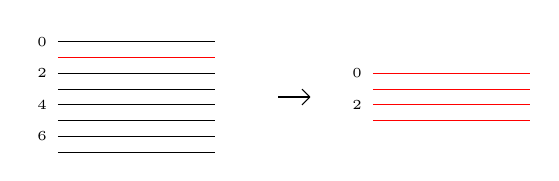
\begin{tikzpicture}
    %LUT
    \node[fill=white, text=black, draw=white] at (-0.2,1.4) {\tiny 0};
    \draw (0,0) -- (2,0);
    \draw (0,0.2) -- (2,0.2);
    \node[fill=white, text=black, draw=white] at (-0.2,1.0) {\tiny 2};
    \draw (0,0.4) -- (2,0.4);
    \draw (0,0.6) -- (2,0.6);
    \node[fill=white, text=black, draw=white] at (-0.2,0.6) {\tiny 4};
    \draw (0,0.8) -- (2,0.8);
    \draw (0,1.0) -- (2,1.0);
    \node[fill=white, text=black, draw=white] at (-0.2,0.2) {\tiny 6};
    \draw[draw=red] (0,1.2) -- (2,1.2);
    \draw (0,1.4) -- (2,1.4);
    
    \draw (2.8,0.7) -- (3.2,0.7);
    \draw (3.1,0.8) -- (3.2,0.7);
    \draw (3.1,0.6) -- (3.2,0.7);

    \node[fill=white, text=black, draw=white] at (3.8,1.0) {\tiny 0};
    \draw[draw=red] (4,0.4) -- (6,0.4);
    \draw[draw=red] (4,0.6) -- (6,0.6);
    \node[fill=white, text=black, draw=white] at (3.8,0.6) {\tiny 2};
    \draw[draw=red] (4,0.8) -- (6,0.8);
    \draw[draw=red] (4,1.0) -- (6,1.0);

    \end{tikzpicture}
    \caption{LUT\#2=16\\00000010$\rightarrow$1111}
    \label{fig:LUT2}
\end{subfigure}
\begin{subfigure}{.45\textwidth}
    \centering
    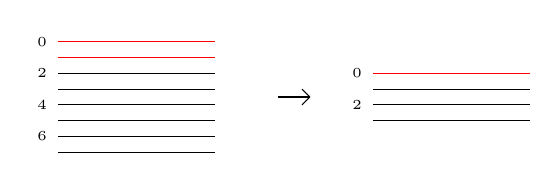
\begin{tikzpicture}
    %LUT
    \node[fill=white, text=black, draw=white] at (-0.2,1.4) {\tiny 0};
    \draw (0,0) -- (2,0);
    \draw (0,0.2) -- (2,0.2);
    \node[fill=white, text=black, draw=white] at (-0.2,1.0) {\tiny 2};
    \draw (0,0.4) -- (2,0.4);
    \draw (0,0.6) -- (2,0.6);
    \node[fill=white, text=black, draw=white] at (-0.2,0.6) {\tiny 4};
    \draw (0,0.8) -- (2,0.8);
    \draw (0,1.0) -- (2,1.0);
    \node[fill=white, text=black, draw=white] at (-0.2,0.2) {\tiny 6};
    \draw[draw=red] (0,1.2) -- (2,1.2);
    \draw[draw=red] (0,1.4) -- (2,1.4);
    
    \draw (2.8,0.7) -- (3.2,0.7);
    \draw (3.1,0.8) -- (3.2,0.7);
    \draw (3.1,0.6) -- (3.2,0.7);

    \node[fill=white, text=black, draw=white] at (3.8,1.0) {\tiny 0};
    \draw (4,0.4) -- (6,0.4);
    \draw (4,0.6) -- (6,0.6);
    \node[fill=white, text=black, draw=white] at (3.8,0.6) {\tiny 2};
    \draw (4,0.8) -- (6,0.8);
    \draw[draw=red] (4,1.0) -- (6,1.0);

    \end{tikzpicture}
    \caption{LUT\#3=1\\00000011$\rightarrow$0001}
\end{subfigure}
\caption[LUT examples]{LUT examples - cases are explained in main text.}
\label{LUTexamples}
\end{figure}


% ******************************* TLB commissioning ****************************
\section{TLB Commissioning}

The first step in using the TLB at FASER is to make sure it respects every specifications. To do this, we install the TLB board in a scintillator laboratory at CERN. The setup to test the board consists of a pulse generator, an oscilloscope, the digitizer\footnote{The digitizer's brand and model are CAEN V1730.} and the TLB, see Fig. \ref{fig:TLBtestSetup}. 

\begin{figure}
  \centering
    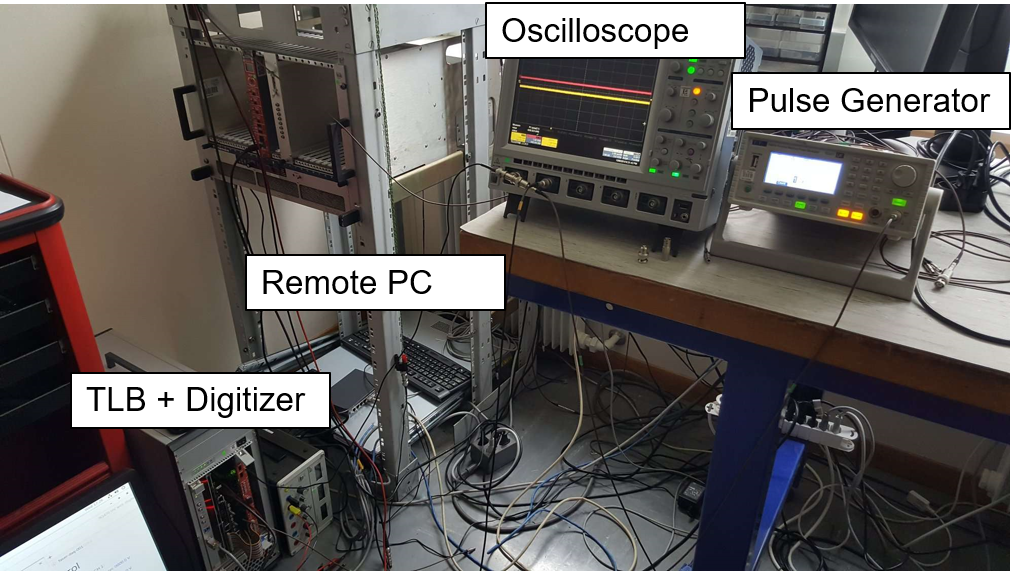
\includegraphics[width=1.0\textwidth]{TLBSetup.png}
    \caption[TLB Test Setup]{TLB Test Setup in the scintillator lab.}
    \label{fig:TLBtestSetup}   
\end{figure}

\subsection{Sampling Phase}

The first element that has been tested is the sampling phase. We want the TLB input signal to be synchronized with the 40MHz LHC clock\footnote{40 MHz or 25 ns between each rise of the clock signal and 12.5 ns between every phase change.} such that a signal is always generated a fixed number of clock cycles after a physics signal. However, because the digitizer outputs at 125 MHz we have an inherent 8 ns jitter \footnote{This is a continuous jitter as opposed to discrete.}. This means that depending on the length of the cable the signal from the digitizer could, for example, fall close to the rising edge of the TLB clock - sometimes triggering, sometimes not. We could however trigger on the falling edge and that would trigger every time because of the length of the digitizer signal (32ns). This is the sampling phase option we need to test. In Fig. \ref{fig:Timing} the incoming physics signal is centered on the fourth rising edge of the clock. However because of the jitter, half of them will not trigger if we trigger on the falling edge but all of them will trigger on the rising edge. 

\begin{figure}[htbp!]
    \centering
    \begin{tikztimingtable}
      LHC Clock 40\,MHz  & 6{1.25C} N(A1) 1{1.25C} N(A2) 1{1.25C} N(A3) 9{1.25C}  \\
      \\
      Jitter -4 ns & 6.75L 3.2H 11.3L \\
      Digitizer Pulse +0 ns & 7.15L 3.2H 10.9L \\
      Jitter +4 ns & 7.5L N(B1) 0.05L 1.2H N(B2) 1.25H N(B3) 0.35H 0.4H 10.5L \\
      \extracode
      \tablerules
      \begin{pgfonlayer}{background}
        \foreach \n in {1,...,3}
          \draw [help lines] (A\n) -- (B\n);
      \end{pgfonlayer}
    \end{tikztimingtable}
    \caption[Sampling Phase Timing Diagram]{Sampling on the falling edge trigger on two different clock cycle whereas sampling on the rising edge trigger only on one clock cycle.}
    \label{fig:Timing}
\end{figure}

To test this, we plug the BCR's \footnote{11245 Hz so $88 \mu s$  between each pulse} output from the TLB to the Digitizer input1 (see Appendix \ref{Panels} \nameref{Panels}, page \pageref{Panels}) as well as into the oscilloscope. We also plug the L1A output from the TLB to the oscilloscope. We then trigger on the L1A. We see that when we trigger on the falling edge, Fig.\ref{fig:SamplingPhaseFalling}, we trigger on two distinct clock cycles whereas if we trigger on the rising edge, Fig. \ref{fig:SamplingPhaseRising}, we only trigger on the same clock cycle. In conclusion, the sampling phase works and the actual setting for FASER will need to be calculated or measured once the FASER assembly is finished. Each input line might have a different setting depending on the length of the cables connecting the trackers to the TLB.

\begin{figure}[htbp!]
\centering
\begin{subfigure}{.5\textwidth}
  \centering
  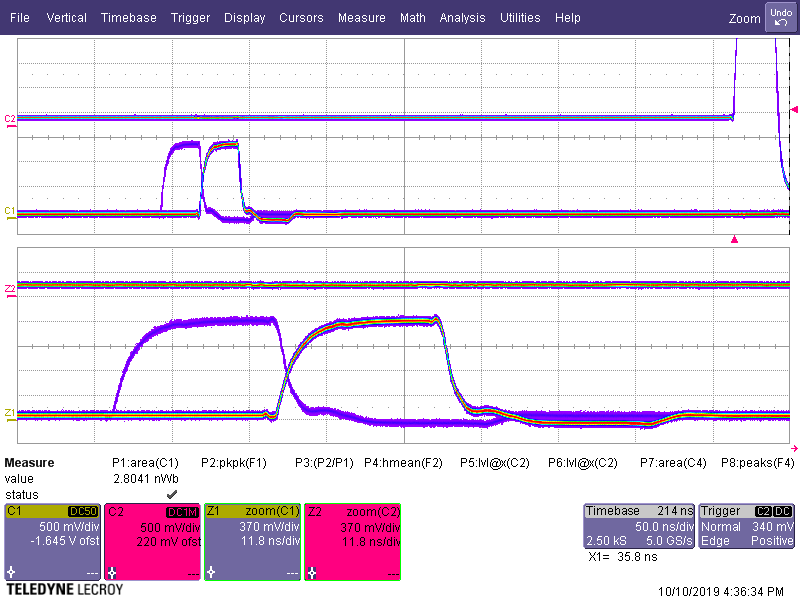
\includegraphics[width=1.0\linewidth]{TLBsamplingPhaseAsynchronous.png}
  \caption{Sampled on the falling edge}
  \label{fig:SamplingPhaseFalling}
\end{subfigure}%
\begin{subfigure}{.5\textwidth}
  \centering
  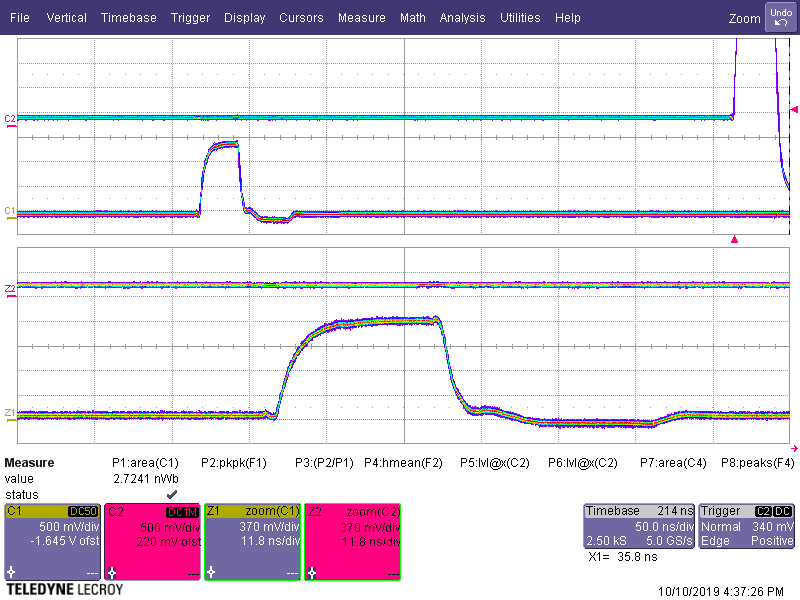
\includegraphics[width=1.0\linewidth]{TLBsamplingPhaseSynchronous.png}
  \caption{Sampled on the rising edge}
  \label{fig:SamplingPhaseRising}
\end{subfigure}
\caption[Sampling Phase]{Sampling on the falling edge we see two distinct signal which means we don't have a reliable time information as opposed to when we sample on the rising edge. The bottom part of each picture is a zoom of the top part. On each top right corner is the L1A the oscilloscope triggers on. The time division on the zoomed part is 11.8 ns/div which makes the signals 25
 ns apart as predicted. The length of the digitizer signal is 32 ns.}
\label{fig:SamplingPhaseResults}
\end{figure}


\subsection{Input Delay}

The next important tuneable setting is the input delay. Because the different detectors are far apart, we must delay the signals that come from the front of FASER. This setting allows the user to delay a signal and to wait for the next incoming signals. This will be useful to coincide all tracking stations throughout the length of FASER. The Fig. \ref{fig:InputDelay} illustrates the concept of event arriving at different clock cycles depending on the travel length. It shows that from the ATLAS IP to FASER we will have a constant time delay of around 64 clock cycles. However, particles will interact with the three tracking stations at different clock cycles, roughly one clock cycle apart (to be determined with actual cable length). The TLB's input delay range is three clock cycles (75 ns) individually adjustable for each 8 channels. This is plenty for the approximately 16.5 ns length of FASER and the additional cabling.

\begin{figure}[htbp!] 
\centering    
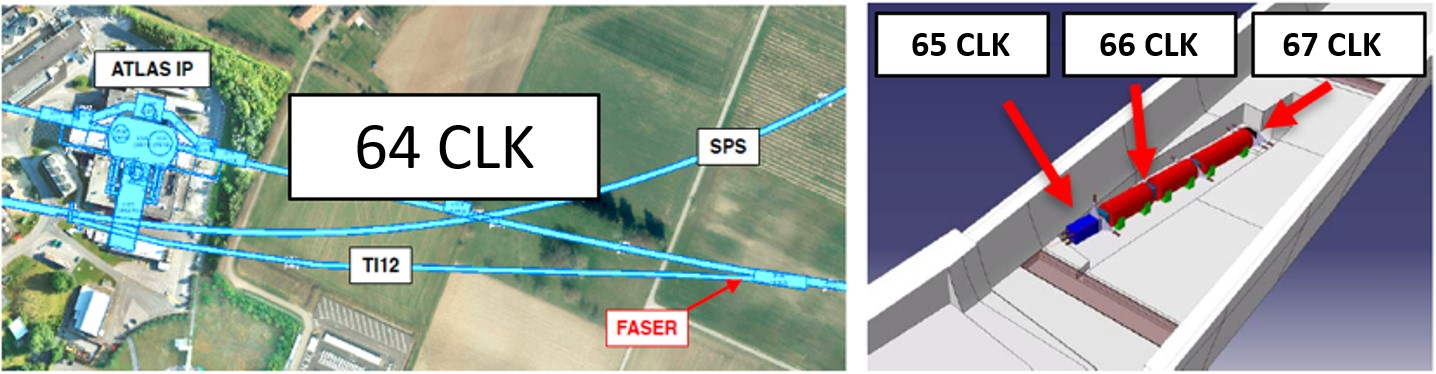
\includegraphics[width=1.0\textwidth]{InputDelayIllustration.jpg}
\caption[Input Delay illustration]{Each physics event will have a constant clock cycle shift depending on where it is located in FASER. Example clock cycle values for illustration purposes.}
\label{fig:InputDelay}
\end{figure}

The test setup, illustrated in Fig. \ref{fig:InputDelaySchema}, had the BCR0 signal from the TLB split with a T-connector into two cables - one 30 ns longer than the other - to the oscilloscope. Both signals then go to the digitizer channel0 and channel2 (the digitizer actually has 16 inputs but every odd channel is merged with the even one) with the 30 ns longer cable going to channel0. What we see on the oscilloscope on Fig. \ref{fig:InputDelayResults} is three signals. In yellow, the C1 delayed signal with respect to the pink C2 and the blue L1A. The test was successful because no L1A were detected if we asked a coincidence on channel0 and channel2 via SC. However, when we delayed the C2 signal by one or two clock cycle (25 - 50 ns) then we would get an L1A which is what happened in Fig. \ref{fig:InputDelayResults}.

\begin{figure}[htbp!]
    \centering
    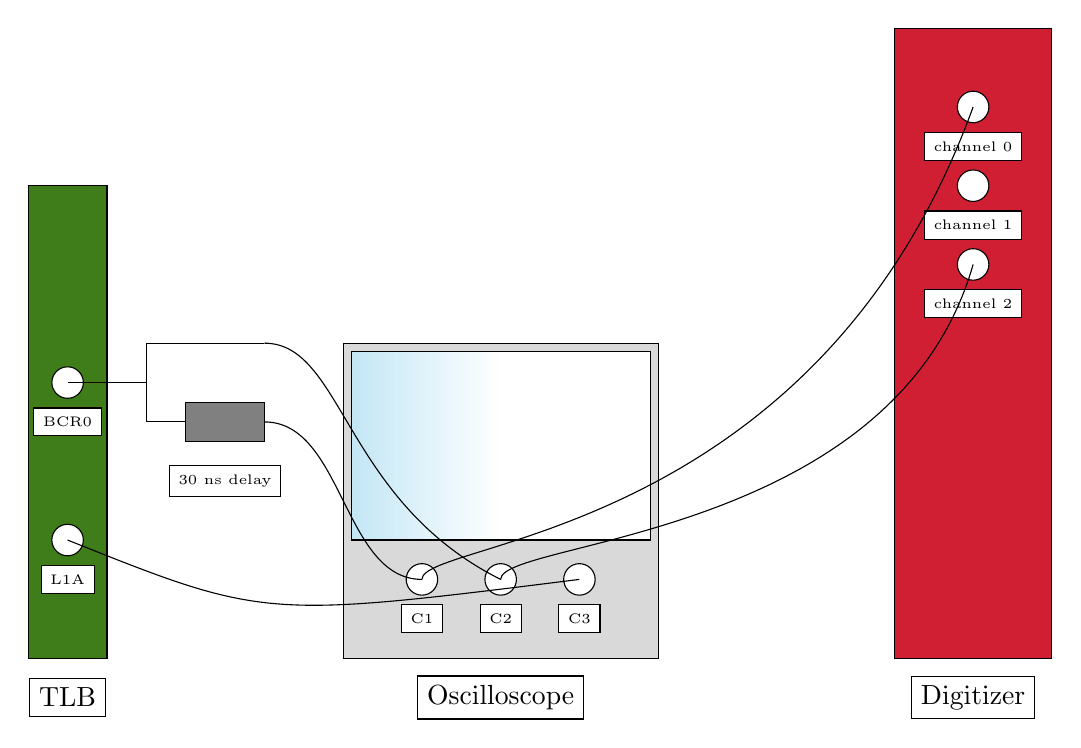
\begin{tikzpicture}
    \definecolor{PCBgreen}{RGB}{41,110,1}
    \definecolor{CustomSky}{RGB}{135,206,235}
    \definecolor{Digitizer}{RGB}{203,5,28}
    \node[draw] at (0.5,-0.5) {TLB};
    \filldraw[fill=PCBgreen!90, draw=black] (0,0) rectangle (1,6);
    \node[fill=white, text=black, draw=black] at (0.5,3.0) {\tiny BCR0};
    \filldraw[fill=white, draw=black] (0.5,3.5) circle (0.2);
    \node[fill=white, text=black, draw=black] at (2.5,2.25) {\tiny 30 ns delay};
    \filldraw[fill=Gray, draw=black] (2,2.75) rectangle (3,3.25); %30ns delay box
    \node[fill=white, text=black, draw=black] at (0.5,1.0) {\tiny L1A};
    \filldraw[fill=white, draw=black] (0.5,1.5) circle (0.2);

    \node[draw] at (6,-0.5) {Oscilloscope};
    \filldraw[fill=Gray!30, draw=black] (4,0) rectangle (8,4);
    \shadedraw[left color=CustomSky!50, right color=White, middle color=White, draw=black] (4.1,1.5) rectangle (7.9,3.9);
    \node[fill=white, text=black, draw=black] at (5,0.5) {\tiny C1};
    \filldraw[fill=white, draw=black] (5,1) circle (0.2);
    \node[fill=white, text=black, draw=black] at (6,0.5) {\tiny C2};
    \filldraw[fill=white, draw=black] (6,1) circle (0.2);
    \node[fill=white, text=black, draw=black] at (7,0.5) {\tiny C3};
    \filldraw[fill=white, draw=black] (7,1) circle (0.2);
    \draw (0.5,1.5) .. controls (3.0,0.5) and (3.0,0.5) .. (7,1);

    \node[draw] at (12,-0.5) {Digitizer};
    \filldraw[fill=Digitizer!90, draw=black] (11,0) rectangle (13,8);
    \node[fill=white, text=black, draw=black] at (12,6.5) {\tiny channel 0};
    \filldraw[fill=white, draw=black] (12,7) circle (0.2);
    \node[fill=white, text=black, draw=black] at (12,5.5) {\tiny channel 1};
    \filldraw[fill=white, draw=black] (12,6) circle (0.2);
    \node[fill=white, text=black, draw=black] at (12,4.5) {\tiny channel 2};
    \filldraw[fill=white, draw=black] (12,5) circle (0.2);
    
    %cabling
    \draw (0.5,3.5) -- (1.5,3.5);
    \draw (1.5,3.5) -- (1.5,4);
    \draw (1.5,4) -- (3,4);
    \draw (1.5,3.5) -- (1.5,3);
    \draw (1.5,3) -- (2,3);
    \draw (5,1) .. controls (5,1.5) and (10.0,1.5) .. (12,7);
    \draw (3,4) .. controls (4,4) and (4,2) .. (6,1);
    \draw (3,3) .. controls (4,3) and (4,1) .. (5,1);
    \draw (6,1) .. controls (6,1.5) and (11.0,1.5) .. (12,5);
    
    \end{tikzpicture}
    \caption[Input Delay schema]{Input Delay Schema. The BCR0 outputs a signal at 11245 Hz which is sent as an input in channel 0 and channel 2. We then see the L1A output. (Not shown on the figure is the LIMO cable connecting the digitizer to the TLB to communicate).}
    \label{fig:InputDelaySchema}
\end{figure}

\begin{figure}[htbp!] 
\centering    
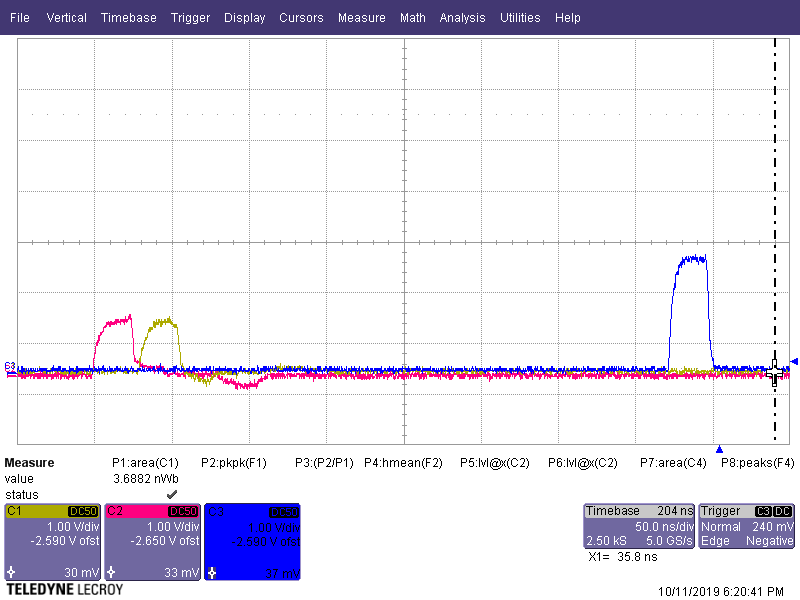
\includegraphics[width=0.7\textwidth]{TLB_Test_30ns_delay.png}
\caption[Input Delay]{Input delay. C1 (yellow) is delayed by 30 ns with respect to C2 (pink). The L1A (blue) is seen because of to the input delay of 1 clock cycle.}
\label{fig:InputDelayResults}
\end{figure}

\subsection{Coincidence Logic Test}

The following test is the coincidence logic test. We took the same setup as in Fig. \ref{fig:InputDelaySchema} but without the 30 ns delay and modified the look up table's value via SC with three different settings presented in Table \ref{table:coincidence}. The first coincidence we tried was to set all the LUT values to 0 and LUT\#1=1. That means we would only get an L1A if signals where received on channel0. In our setup we could unplug channel2 and still get L1As, however, if one were to unplug channel0 there wouldn't be any L1A as planned. Next is LUT\#2=1, this means that the TLB would only send an L1A if the digitizer received a signal in channel2. This worked as expected and even with channel0 unplugged one got signals. The last test was to set LUT\#3=1 and everything else to zero. This means requesting a coincidence from channel0 and channel2. As a result, L1As only got sent if channel0 and channel2 received a signal on the same clock cycle. Unplugging any one of the channels stopped the L1A generation.

\begin{table}[htbp!]
\caption{Look up table setting for the coincidence logic test}
\centering
\label{table:coincidence}
\begin{tabular}{l c c c c c c}
\toprule
LUTArray & \#0 & \#1 & \#2 & \#3 & \#n & \#255 \\
\midrule
Triggers on ch0 & 0 & 1 & 0  & 0 & ... & 0 \\
Triggers on ch2 & 0 & 0 & 1  & 0 & ... & 0 \\
Coincidence on ch0 and ch2 & 0 & 0 & 0  & 1 & ... & 0 \\
\bottomrule
\end{tabular}
\end{table}

\subsection{Prescales}
\label{Prescales}

Prescales allows to sample the incoming data by selecting only a fraction of it. For example if you set prescale to 2 then only every 2nd trigger is passed, for a prescale of 3 only every 3rd signal is passed and so on. To test if the prescales where working, we sent fixed pulses with a signal generator - Fig.\ref{fig:SignalGenerator} - at 2 kHz with a signal width of 40 ns and 1 Volt peak to peak. Table \ref{table:prescale} contains data taken from the TLB's GUI. As expected the time to fill increase by two and seven-fold with the prescale setting. Additional tests, using the oscilloscope to visualize, were performed and can be seen on Fig. \ref{fig:Prescales}. The yellow signal on channel1, C1, represents the pulse generator whereas the pink signal C2 represents the L1As. In  Fig.\ref{fig:2kHzPrescale1} yellow and pink signals overlap because for every pulse sent, an L1A is emitted. However for Fig.\ref{fig:2kHzPrescale2} one in two signals gets vetoed by the prescale setting and in Fig. \ref{fig:2kHzPrescale3} one in three.

\begin{table}[htbp!]
\caption{Prescale table for a pulse frequency of 1[kHz] and a width of 40 ns. Time values are to fill a 1024KB file.}
\centering
\label{table:prescale}
\begin{tabular}{c c c c c}
\toprule
Prescale setting & Time to fill [h:m:s] & T [s] & \# events & L1A frq [Hz] \\
\midrule
1 & 00:00:52 & 52 & 52432 & 1008.31 \\
2 & 00:01:45 & 105 & 52432 & 499.35 \\
7 & 00:06:07 & 367 & 52430 & 142.86 \\
\bottomrule
\end{tabular}
\end{table}


\begin{figure}[htbp!] 
\centering    
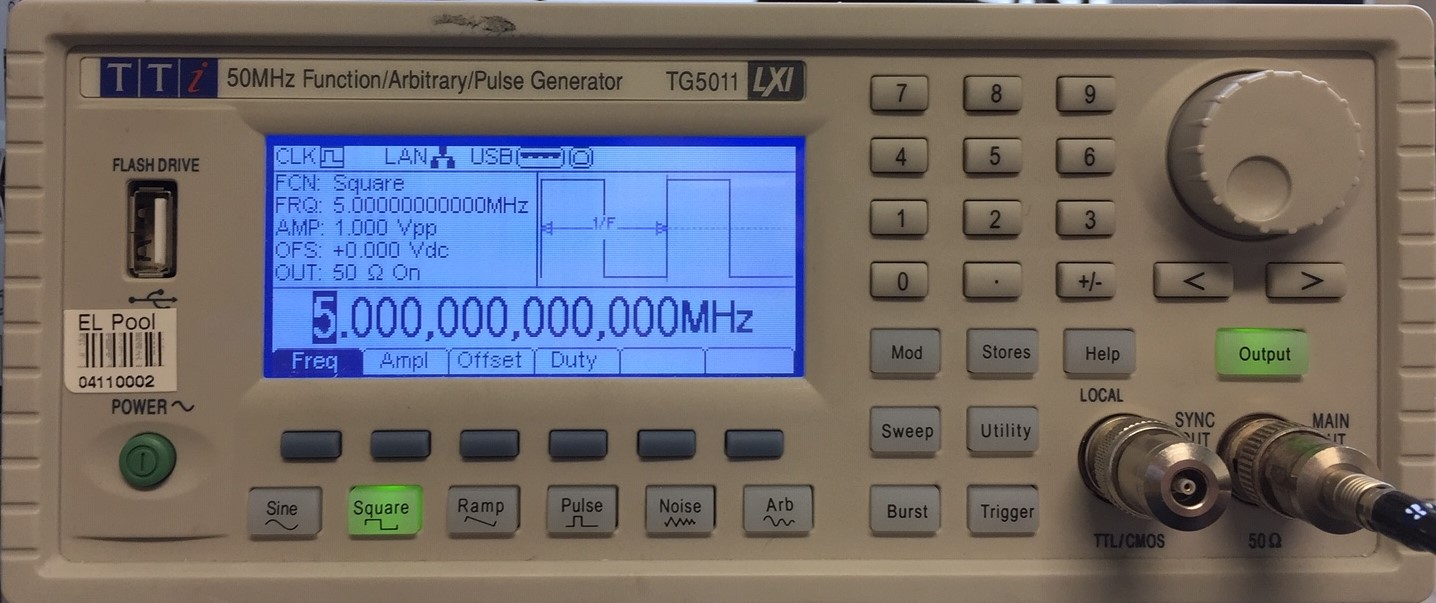
\includegraphics[width=0.6\textwidth]{SignalGenerator5Mhz.jpg}
\caption[Signal Generator]{Signal generator installed in the scintillator lab used to generator pulses that mimic physics signal.}
\label{fig:SignalGenerator}
\end{figure}

\begin{figure}
    \centering
    \begin{subfigure}[t]{.5\textwidth}
      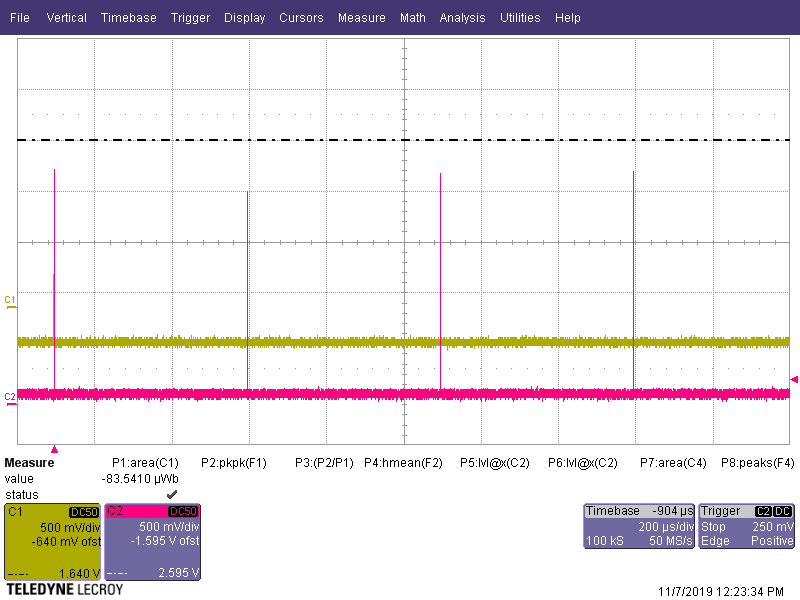
\includegraphics[width=1.0\linewidth]{2kHzPrescale1.png}
      \captionsetup{width=0.8\textwidth}
      \caption{Prescale set to 1 - Every event from the pulse generator is level 1 accepted.}
      \label{fig:2kHzPrescale1}
    \end{subfigure}%
    \begin{subfigure}[t]{.5\textwidth}
      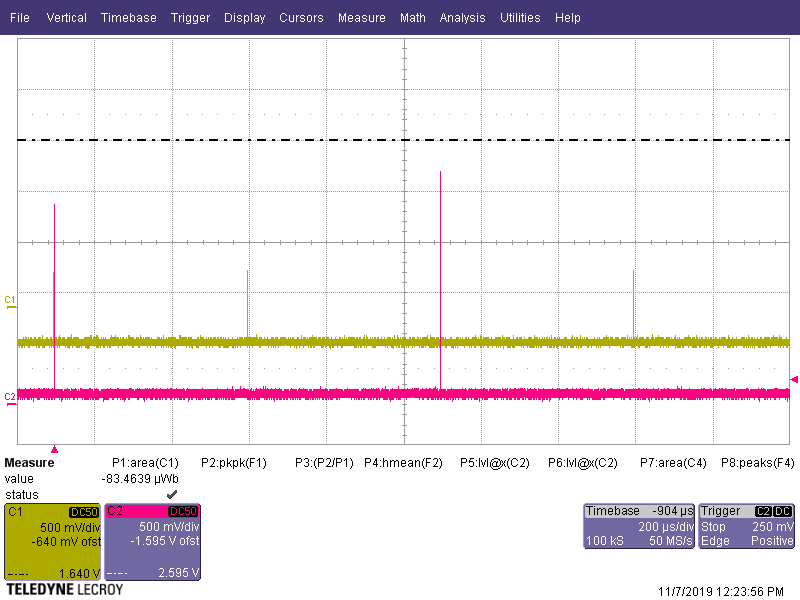
\includegraphics[width=1.0\linewidth]{2kHzPrescale2.png}
      \captionsetup{width=0.8\textwidth}
      \caption{Prescale set to 2 - One in two events get vetoed.}
      \label{fig:2kHzPrescale2}
    \end{subfigure}
    \begin{subfigure}[t]{.5\textwidth}
      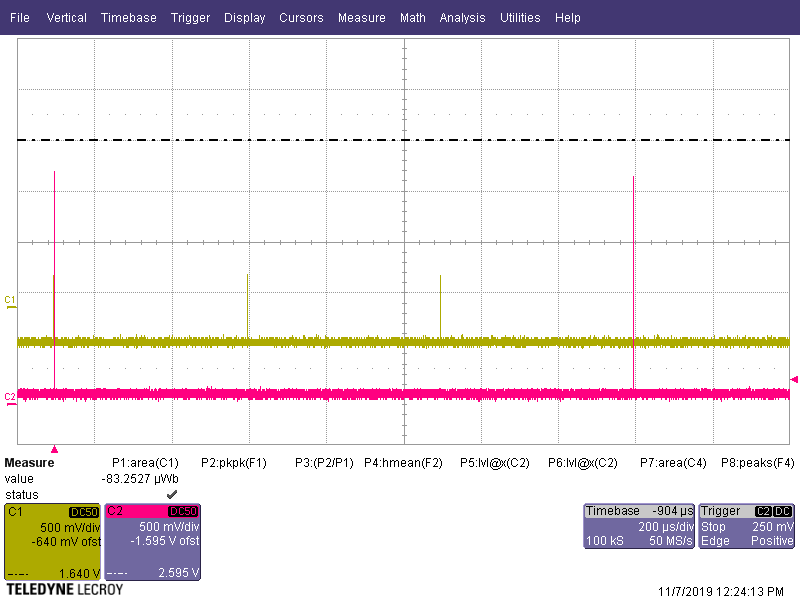
\includegraphics[width=1.0\linewidth]{2kHzPrescale3.png}
      \caption{Prescale set to 3 - One in three events get vetoed.}
      \label{fig:2kHzPrescale3}
    \end{subfigure}
    \caption[Prescale results]{Prescale results - the yellow signal is the pulse generator, the pink signal is the L1A.}
    \label{fig:Prescales}
\end{figure}


\subsection{Random Trigger}
\label{Random Trigger}

Random triggers are a pseudo-random generator generating 25 ns wide pulses (TBP5) at a user-settable (SC) average pulse rate of about 10-1000Hz. It is a unique input line that has 8 different settings ranging from 0 to 7. In our test we tried 3 different settings shown in Table \ref{table:RandomTrigger}. We see that the frequencies range from 20-360Hz close to what was specified in the TLB specifications\footnote{A setting of 0 is actually the highest frequency one can set and should be even higher in frequency}. Another measurements made was the time between two outgoing L1As shown in Fig. \ref{fig:RandomGenerator}. We see for these two settings that the distribution is indeed random as intended.

\begin{figure}[htbp!] 
\centering    
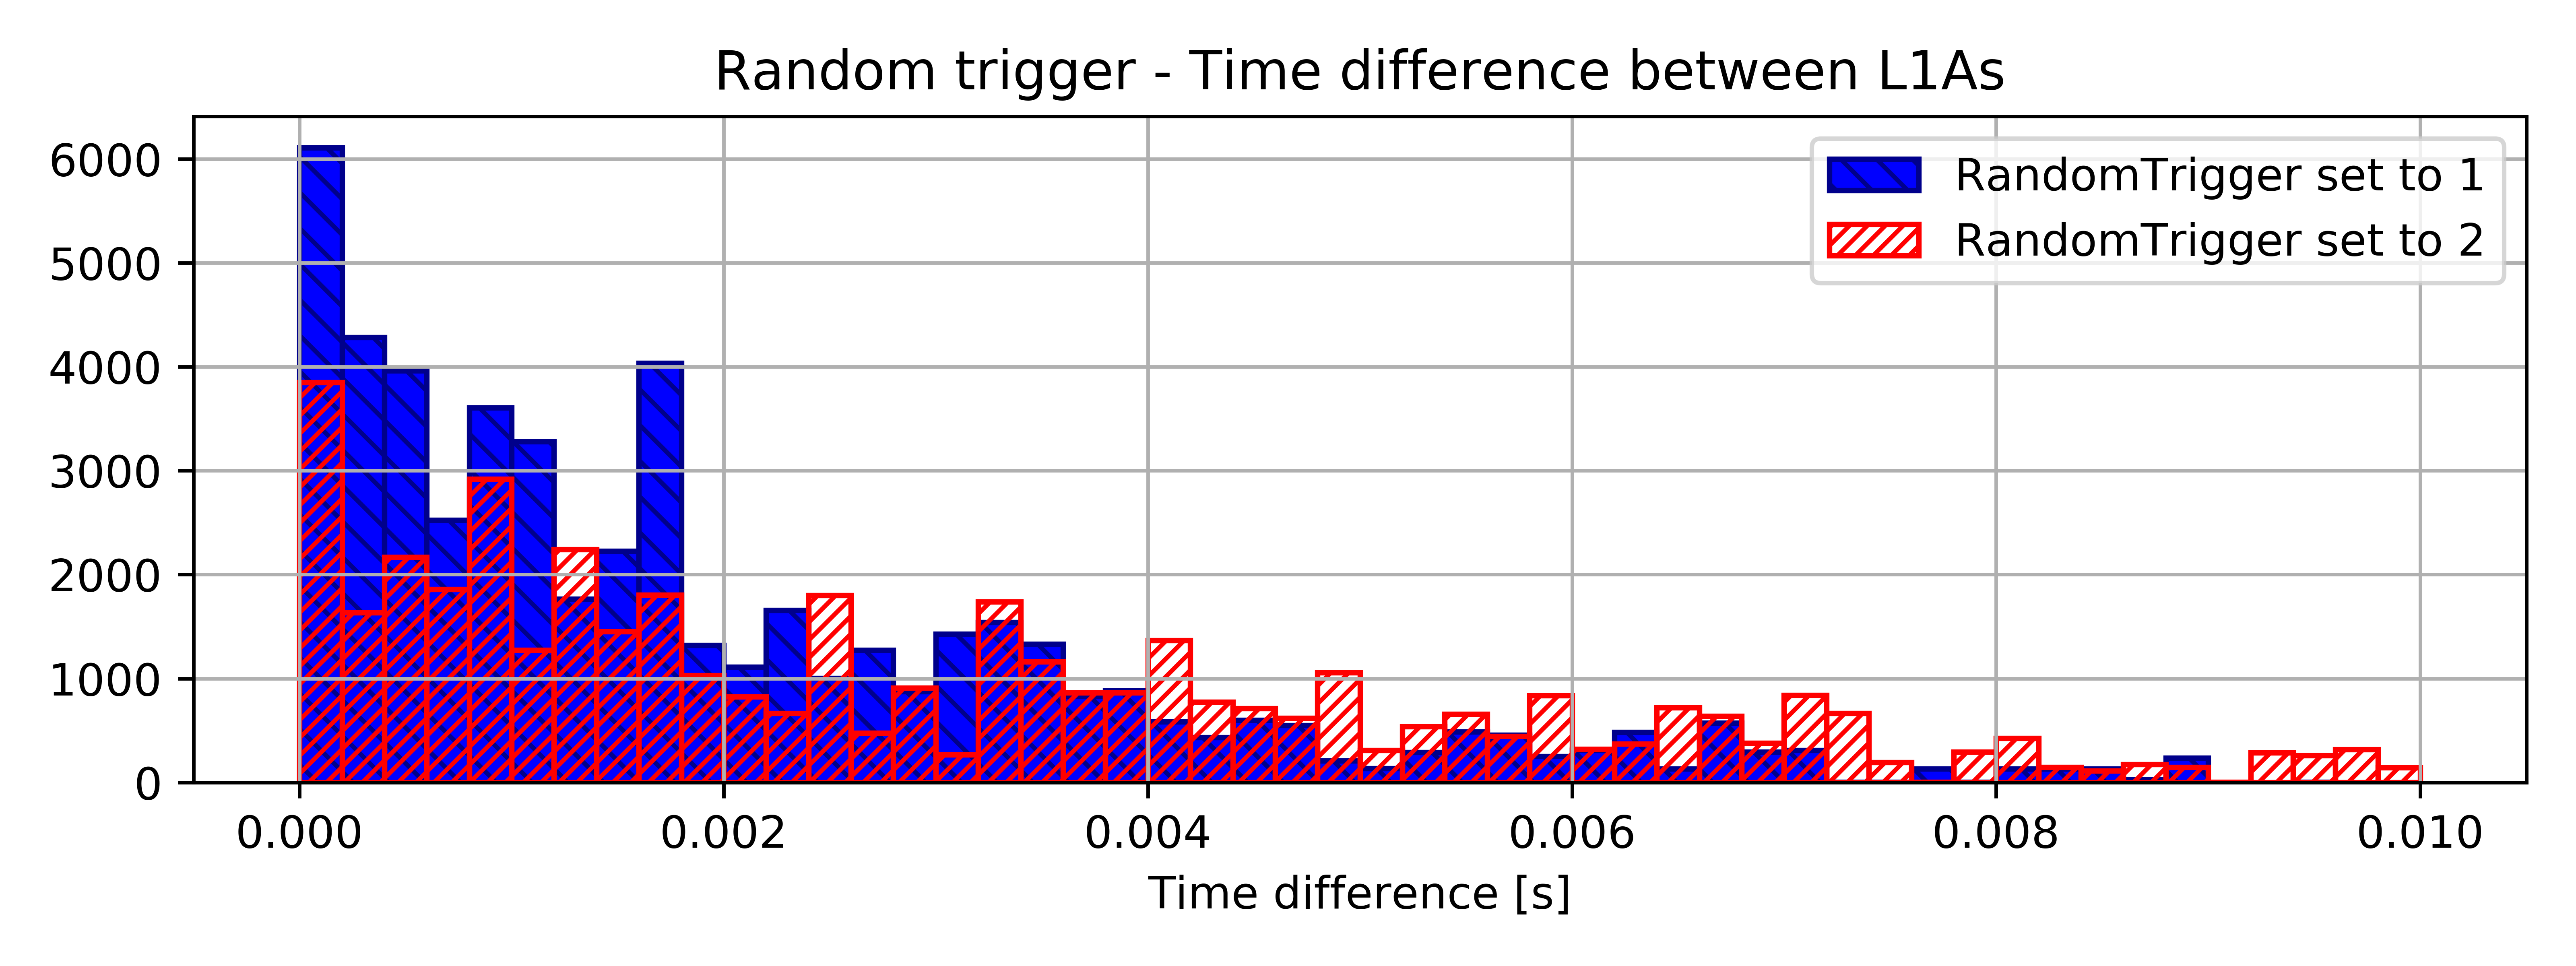
\includegraphics[width=\textwidth]{Raster/RandomTriggerTimeDifferences.png}
\caption[Random Trigger]{The Random Generator has eight different settings from 0 to 7. 0 correspond to the fastest trigger rate and 7 to the lowest.}
\label{fig:RandomGenerator}
\end{figure}

\begin{table}[htbp!] 
\caption{Random trigger table. Time values are to fill a 1024KB file.}
\centering
\label{table:RandomTrigger}
\begin{tabular}{c c c c}
\toprule
Random setting & Time to fill [h:m:s] & Avg time btwn triggers [s] & Avg frq [Hz] \\
\midrule
1 & 1.71 & $2.78\cdot10^{-3}$ & 359 \\
2 & 4.37 & $4.25\cdot10^{-3}$ & 235 \\
7 & 12.8 & $4.83\cdot10^{-2}$ & 20.7 \\
\bottomrule
\end{tabular}
\end{table}

\subsection{Software Trigger}
\label{Software Trigger}

Software trigger is an additional trigger line that is user settable. For this module testing, we simply sent 10 software triggers via the GUI, see Fig. \ref{fig:SoftwareTriggerGUI}, while taking data. This gives the plot on Fig. \ref{fig:SoftwareTriggerGraph} which shows the ten software triggers. The x-axis represents the time it took to send the different trigger signals.

\begin{figure}[htbp!] 
\centering  
    \begin{subfigure}[t]{.4\textwidth}
    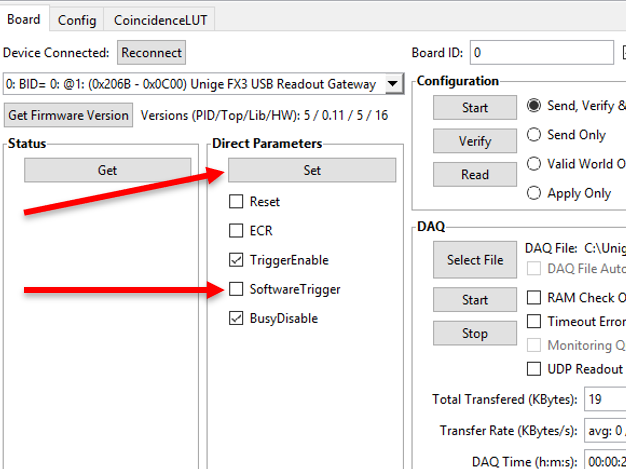
\includegraphics[width=1.0\textwidth]{SoftwareTrigger.png}
    \captionsetup{width=0.8\textwidth}
    \caption{GUI procedure.}
    \label{fig:SoftwareTriggerGUI}
    \end{subfigure}
    \begin{subfigure}[t]{.4\textwidth}
    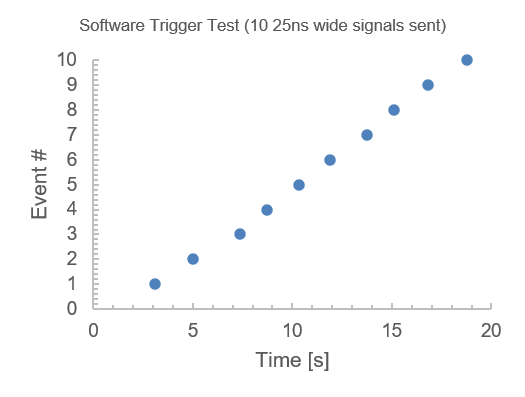
\includegraphics[width=1.0\textwidth]{SoftwareTriggerGraph.png}
    \captionsetup{width=0.8\textwidth}
    \caption{Software Trigger as a function of time.}
    \label{fig:SoftwareTriggerGraph}
    \end{subfigure}
\caption[Software Trigger results]{Software Triggers can be used as manual sources of trigger (and L1A) if no detector is set as an input.}
\label{SoftwareTrigger}
\end{figure}

\subsection{Deadtime from the Rate Limiter}

By design the TLB's rate is limited to three L1As per 15 orbits to protect from noisy triggers. This means that if you feed the BCR signal you'll only get an L1A every 5 orbits. This is what was tested on Fig. \ref{fig:SamplingRate}. The yellow signal on C1 is the BCR signal at 11.245 kHz and the pink signal are the L1As at 2.249 kHz \footnote{Calculation: $\frac{3}{15\cdot\frac{1}{11245}}=2.249 kHz$}. As expected we see a pink L1A every 5 yellow BCR because of the vetoing.

\begin{figure}[htbp!] 
\centering    
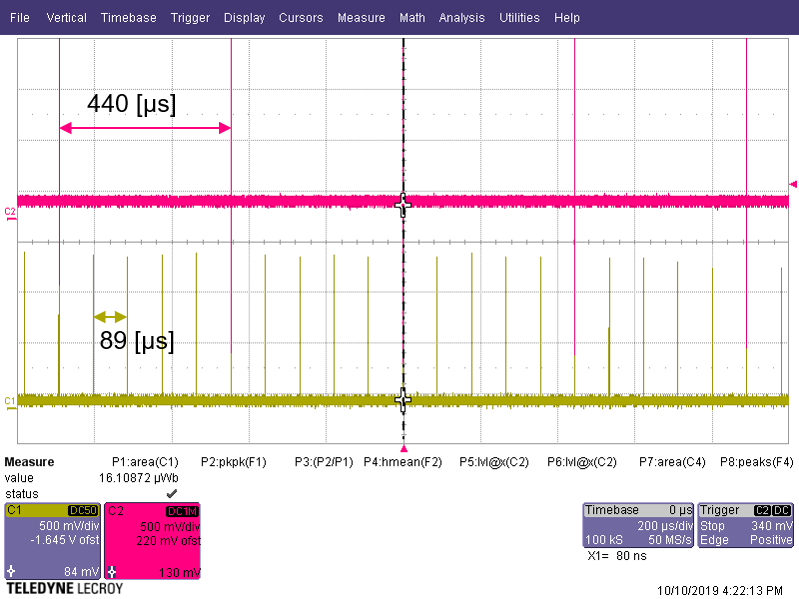
\includegraphics[width=0.6\textwidth]{SamplingRate.png}
\caption[Sampling Rate results]{Sampling Rate results - In yellow the TLB receives a BCR signal at 11.245 kHz. As the rate limiter kicks in, only 1 out of 5 trigger signal outputs an L1A.}
\label{fig:SamplingRate}
\end{figure}

\subsection{Simple Deadtime}

To test the simple deadtime, we generate with the pulse generator 10 Mhz pulses with 10 cycles, 40 ns width and 1 volt peak to peak. On Fig. \ref{fig:Deadtime0} we see the three L1As in pink. There are only three because of the rate limiter is kicking in. They are at the same frequency as the driving signal with a phase because of the processing and cable length. Setting the simple deadtime parameter to 10 in Fig.\ref{fig:Deadtime10} results in the L1As being separated by 10 clock cycles or 250 ns as expected.

\begin{figure}[htbp!] 
\centering    
    \begin{subfigure}[t]{.4\textwidth}
    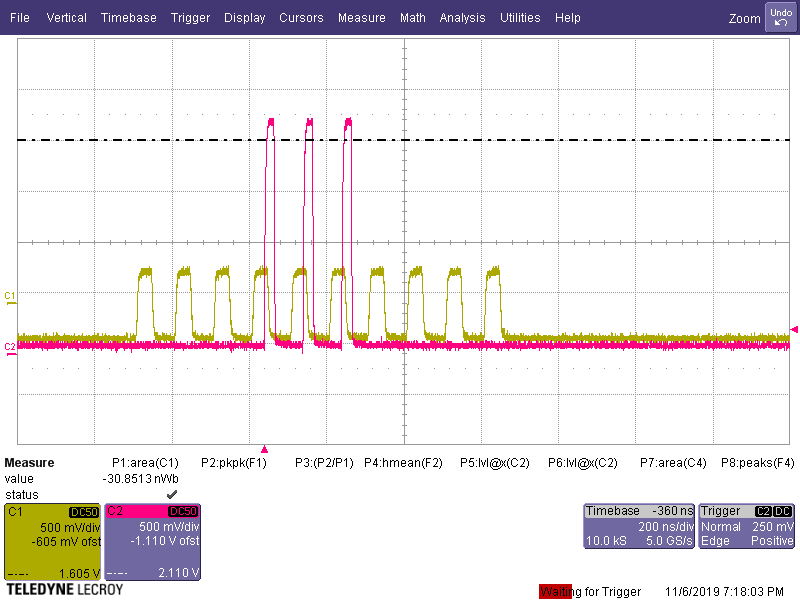
\includegraphics[width=1.0\textwidth]{DeadtimeSet0.png}
    \caption{Deadtime set to 0.}
    \label{fig:Deadtime0}
    \end{subfigure}
    \begin{subfigure}[t]{.4\textwidth}
    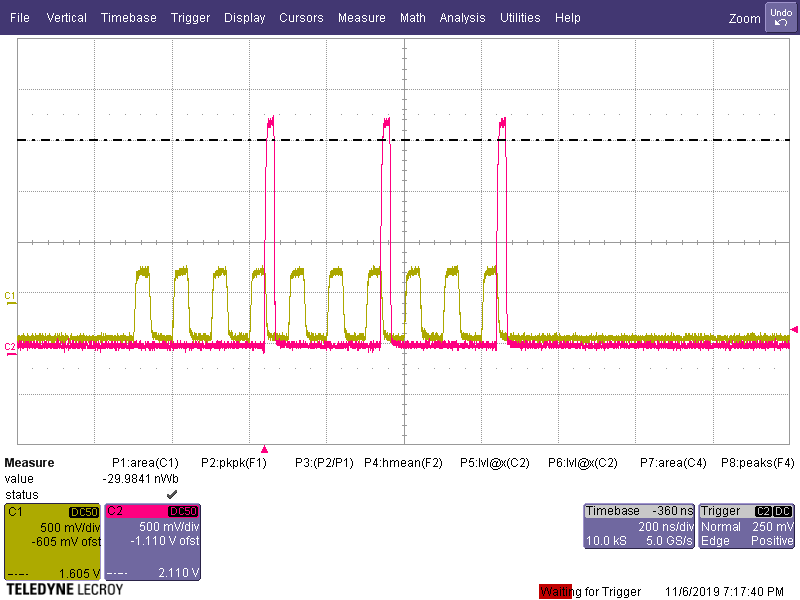
\includegraphics[width=1.0\textwidth]{DeadtimeSet10.png}
    \caption{Deadtime set to 10.}
    \label{fig:Deadtime10}
    \end{subfigure}
\caption[Deadtime results oscilloscope]{Deadtime results - Changing the deadtime parameter forces the TLB to veto during the number of clock cycle selected.}
\label{fig:Deadtime}
\end{figure}

\subsection{Deadtime from the BCR veto}

\nomenclature[z-BCID]{BCID}{Bunch Counter Identifier}

The deadtime manager takes care of vetoing L1As via multiple criterium. One of them is that an L1A cannot be too close the a BCR. This behaviour is well described in the specifications. "A veto signal is generated if a BCR was sent in the last 6 CLKs, this CLK or the next two CLK cycles, i.e, if BCR-3 is set in the last 9 CLK cycles". The orbit delay generates the BCR-3 three CLK cycles earlier. In this test we are sending a pulse signal of 1[kHz], width 40ns and 1 Volt peak to peak and we fill a 10'000KB file with L1As. In Fig.\ref{fig:DeadtimeBig} we plot the BCID range from 0 to 3563. We find while zooming in on the beginning in Fig.\ref{fig:DeadtimeBeginning} and on the end in Fig. \ref{fig:DeadtimeEnd} that it actually goes from 3 to 3557 and that we are missing 9 BCIDs as expected.

\begin{figure}[htbp!] 
\centering    
    \begin{subfigure}[t]{1.0\textwidth}
    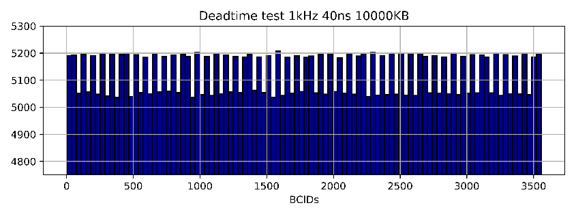
\includegraphics[width=1.0\textwidth]{DeadtimeManagerBig.png}
    \caption{Deadtime Manager whole range.}
    \label{fig:DeadtimeBig}
    \end{subfigure}
    \begin{subfigure}[t]{.4\textwidth}
    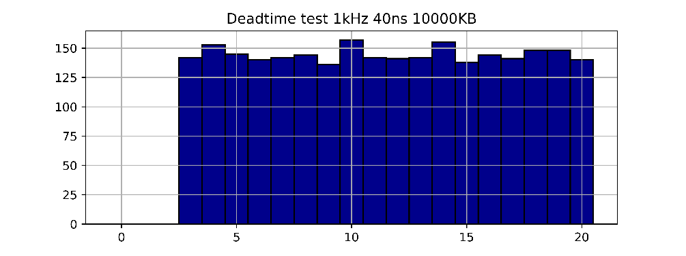
\includegraphics[width=1.0\textwidth]{DeadtimeManagerFront.png}
    \caption{Deadtime zoomed on beginning.}
    \label{fig:DeadtimeBeginning}
    \end{subfigure}
    \begin{subfigure}[t]{.4\textwidth}
    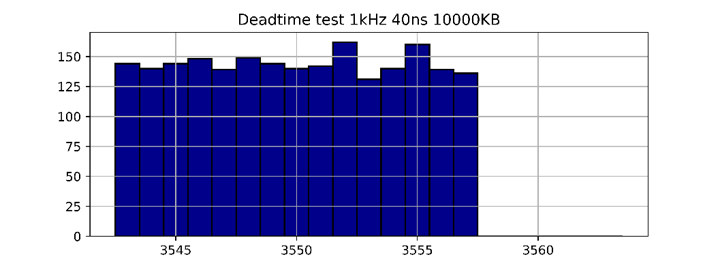
\includegraphics[width=1.0\textwidth]{DeadtimeManagerEnd.png}
    \caption{Deadtime zoomed on the end.}
    \label{fig:DeadtimeEnd}
    \end{subfigure}
\caption[Deadtime results histogram]{Deadtime results.}
\label{fig:DeadtimeManager}
\end{figure}

Another thing we are able to see in the output data are the sources of veto. For example in Fig. \ref{fig:VetoSources} we read the monitoring data for 11245 BCRs with the deadtime setting set to 10, the frequency of the signal generator set to 10 MHz, 100 pulses with a pulse period of 11 ns and a width of 40 ns. We are then able to see the simple deadtime, the BCR deadtime, the busy tracker (not working in our setup because no tracker connected) and the rate limiter.

\begin{figure}[htbp!] 
\centering    
\includegraphics[width=0.6\textwidth]{MonitoringData11245HzDeadtime10Frq10MHZ100pulsePlsPrd100nsWidth40ns.png}
\caption[Veto sources]{Able to read 4 sources of veto. Pay attention to the vertical axis - bottom one is log scale. (The trackers weren't connected in this setup so the Tracker Busy is flat).}
\label{fig:VetoSources}
\end{figure}

\subsection{Output Delay}

The Output delay consists of delaying the outgoing L1A signal from the TLB. "It is a programmable delay for sending L1A signals at the right latency for each readout output. Each output delay is individually set by SC in CLK counts (7bits)". The option in the GUI is labelled DigitizerDelay and we tried three different options presented in Table \ref{table:Outputtable}. The results can be seen on Fig. \ref{fig:OutputDelay}. From left to right we see the first signal has the 16 clock cycle delay which corresponds to 400 ns, the second pulse is with the 4 clock cycle delay which corresponds to 100 ns and the third pulse is with no delay. We see the inherent delay from computing which is roughly 100 ns.

\begin{table}
\caption{Output delay.}
\centering
\label{table:Outputtable}
\begin{tabular}{c c}
\toprule
Digitizer setting [CLK cycles] & Delay [ns] \\
\midrule
0 & 0\\
4 & 100\\
16 & 400\\
\bottomrule
\end{tabular}
\end{table}

\begin{figure}[htbp!] 
\centering    
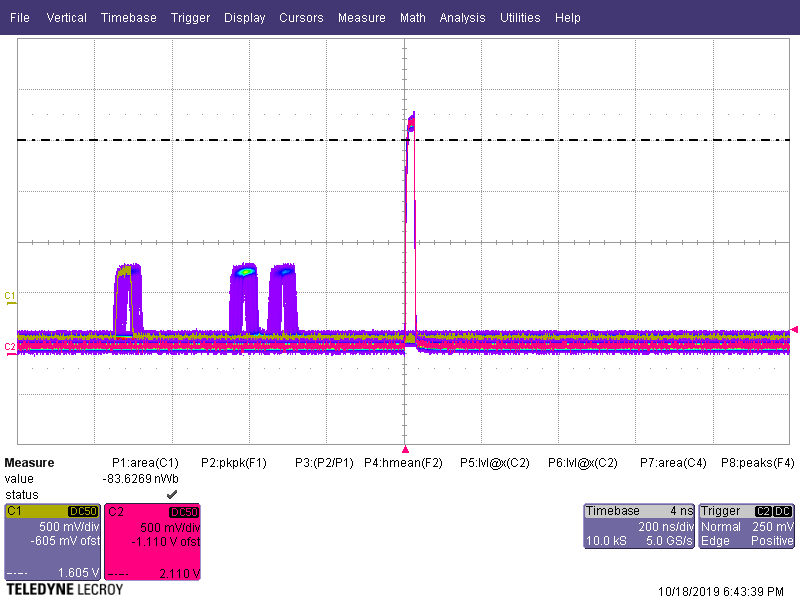
\includegraphics[width=0.7\textwidth]{Digitizer_Delay.png}
\caption[Output Delay]{Output delay with persistence on. Triggering on L1A allows to see the different delays.}
\label{fig:OutputDelay}
\end{figure}

%*******************************************************************************
%****************************** TLB Software *********************************
%*******************************************************************************

\chapter{TLB Software}

Both the TLB and the TRB use the same design of GPIO board and thus the low-level control software is shared. In what follows, the TRB software is introduced and its modifications into TLB software are explained.

\begin{figure}[htbp!] 
\centering    
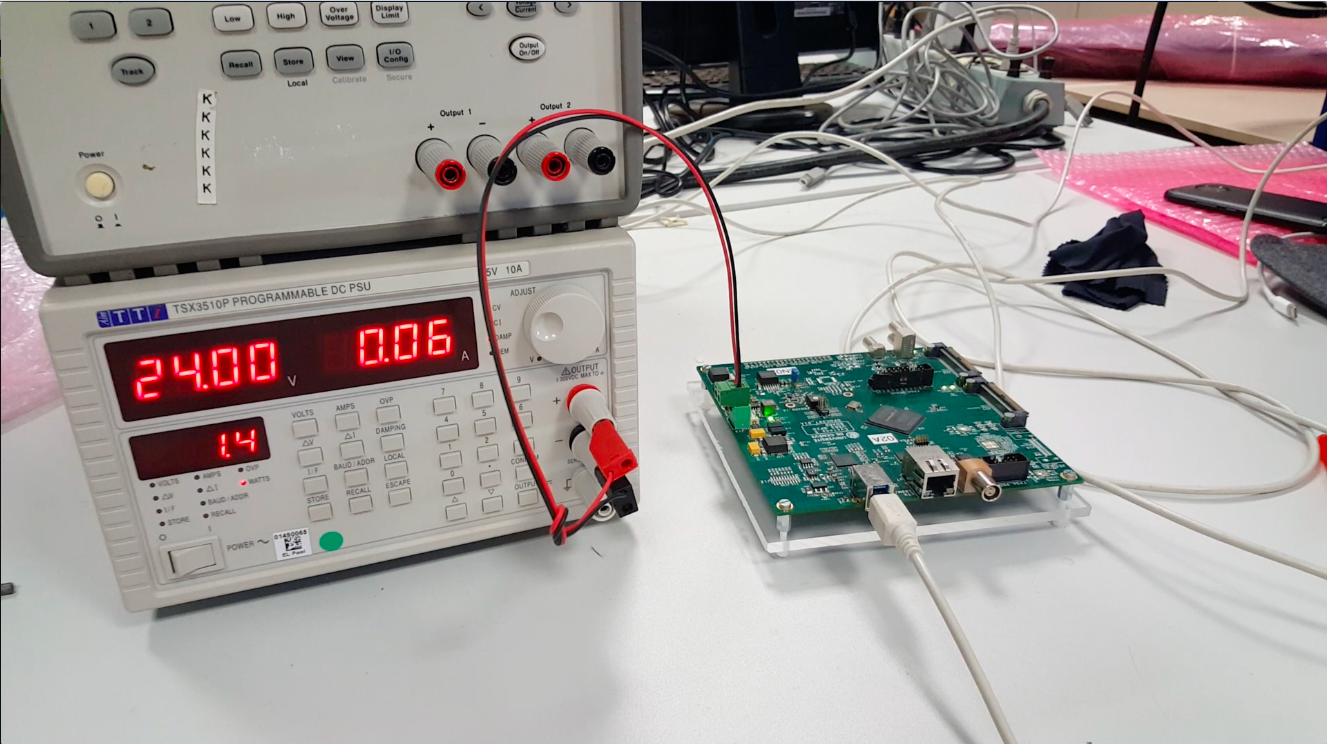
\includegraphics[width=0.6\textwidth]{ChapterDAQ/Figs/Software/TLBwithPowerSupply.png}
\caption[TRB lab set-up]{TRB lab set-up in building 161, CERN, the TRB is powered via the generator with 24.0 V and 0.06 A and connected via USB 3.0 to a laptop for connection tests.}
\label{fig:TRBbdg161Setup}
\end{figure}


\section{TRB/TLB communication program structure}

To send instructions to the board, the GPIO base class is used. This contains the most important function called SendAndRetrieve. It allows the user to change bits at a certain address in memory. A typical program structure to access either the TLB or TRB would be. 

\begin{lstlisting}[caption={In this example, SendAndRetrieve has two parameters: 0x02 and 0x1. 0x02 corresponds to the address in memory and 0x01 corresponds to the payload.},captionpos=b]
#include "../TrackerReadout/GPIOBaseClass.h"
using namespace FASER;
int main() 
{
GPIOBaseClass * MyGPIOAccess = new GPIOBaseClass(false);
MyGPIOAccess->SendAndRetrieve(0x02, 0x1);
return 0;
}
\end{lstlisting}

The SendAndRetrieve command expects the following arguments. \begin{lstlisting}
bool GPIOBaseClass::SendAndRetrieve(uint8_t CmdID, uint16_t CmdArg, uint16_t* AnswArg)
\end{lstlisting}
The first argument "CmdID" is the address in memory and tells the board where to write the second argument "CmdArg" which is the actual bit to change. The last argument "AnswArg" is what the program will write into when it receives something back from the board. In general it will send back the CmdID unless it is requesting specific data. A good check is to verify after each SendAndRetrieve that CmdID == AnswArg.

\section{Configuration json}
\label{configuration}

The full DAQ config will be stored in single json files and the setup can be modified either by directly changing it or via a GUI interaction, see Fig.\ref{fig:ConfigurationJSON}. Most of the configuration will be in this file. The trigger configuration data will be stored on a separate file which can be linked from the main configuration. During each run the configuration used will need to be archived for offline analysis either via common DAQling solution or via a simple text blob in database indexed by run-number.

\begin{figure}[htbp!] 
\centering    
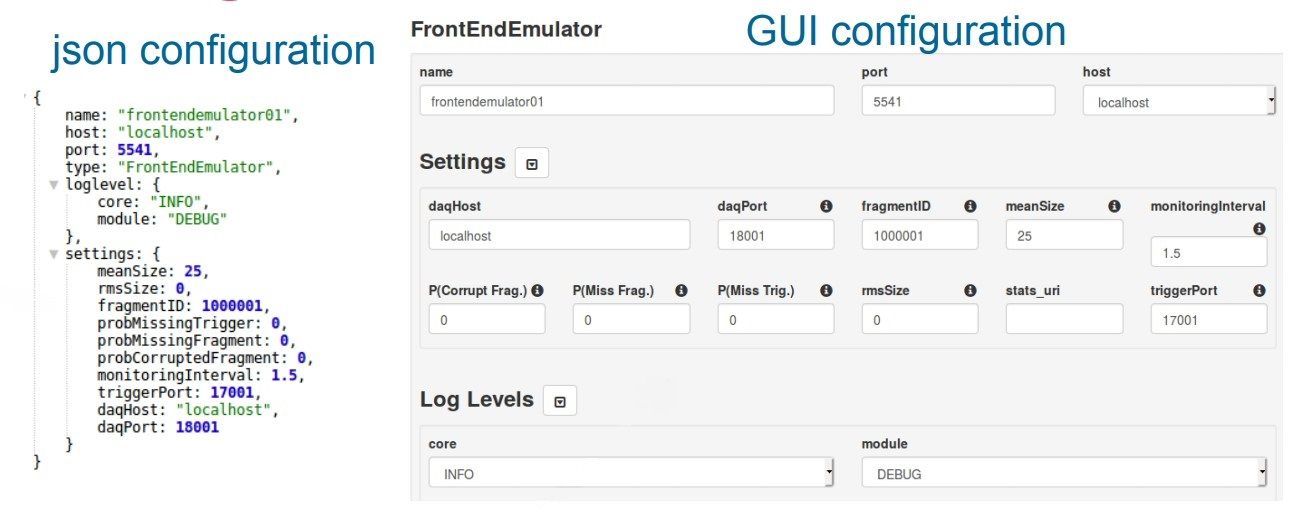
\includegraphics[width=0.6\textwidth]{ChapterDAQ/Figs/GeneralDAQ/configuration.jpg}
\caption{Json and GUI configuration.}
\label{fig:ConfigurationJSON}
\end{figure}


% ******************************* Software Contribution ****************************
\section{Software contribution}

My contribution to the software has been on two fronts: implementation of both the TLB readout and TLB receiver DAQ software. 

\subsection{GPIODrivers}

The GPIODrivers sub-folder located in the main FASER DAQ repository (\href{https://gitlab.cern.ch/faser}{gitlab.cern.ch/faser}) is a package that contains the readout libraries as well as the standalone driver programs for the UniGe GPIO boards used within the FASER experiment's trigger and readout system, namely the Trigger Logic Board and the Tracker Readout Board. Each readout library depends on the GPIOBaseClass library, the base library to access a UniGe GPIO board\footnote{Faser internal information: \href{https://espace.cern.ch/faser-share/Shared\%20Documents/Trigger,\%20DAQ\%20and\%20DCS/Unige\%20FrontEnd\%20Interface\%20-\%20UFE_Protocol-v1.4.pdf}{GPIO front-end interace specifications on sharepoint}}, which is contained in the package.

\begin{figure}[htbp!]
    \centering
    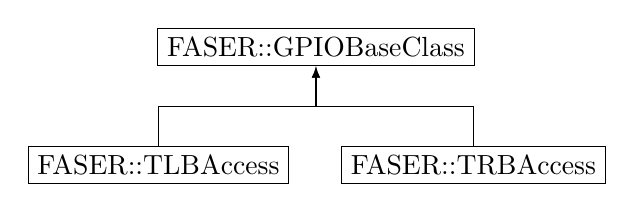
\begin{tikzpicture}
    \node[draw] at (0,0) (A) {FASER::GPIOBaseClass};
    \node[draw] at (-2,-1.5) (B) {FASER::TLBAccess};
    \node[draw] at (2,-1.5) (C) {FASER::TRBAccess};
    \draw[-latex] (B.north) -- ++ (0,0.5) -| (A.south);
    \draw[-latex] (C.north) -- ++ (0,0.5) -| (A.south);
    \end{tikzpicture}
    \caption{GPIOBaseClass inheritance diagram.}
    \label{fig:GPIOBaseClass}
\end{figure}

The TLBAccess\footnote{\href{https://faserdaq.web.cern.ch/faserdaq/gpiodrivers/doc/html/class_f_a_s_e_r_1_1_t_l_b_access.html\#ada95a891d48b8d907e49e51ec3a6d5de}{TLBAccess's documentation.}} is an API to communicate with the Trigger Logic Board included in the above package. It inherits from the GPIOBaseClass and mostly uses the SendAndRetrieve command described earlier. A typical use of the library would be to parse a json configuration file and store it as a variable.

\lstinputlisting[language=C++,caption={Example json configuration format used to configure the TLB.},captionpos=b]{ChapterDAQ/Code/TLBAccess_config_TLBConfiguration.JSON}

The user would then pass the stored parsed json to the ConfigureAndVerifyTLB(json) function that "cleans" the board, i.e. sets all configuration memory bits to zero and sends the configuration. After that, it also verifies if the configuration has been applied correctly. If the configuration has failed it will try again to configure the board. ConfigureAndVerifyTLB() is a large function that uses different functions such as CleanConfig() and ConfigureTLB(). A diagram presenting it's functionnality is shown on Fig. \ref{fig:ConfigureAndVerifyTLB()}.

\begin{figure}[htbp!]
    \centering
    \begin{tikzpicture}[node distance=1.5cm, every node/.style={scale=0.8}]
    \node (start) [startstop] {ConfigureAndVerifyTLB(json)};
    \node (in1) [io, left of=start, text width=2.5cm, xshift=-3.2cm] {Input: json config};
    \node (dec1) [decision, below of=start, text width=3cm] {Was configuration successful ?};
    \node (proc1) [process, right of=dec1, xshift=2.8cm] {ConfigureTLB(json)};
    \node (proc2) [process, below of=proc1, xshift=2.8cm] {CleanConfig()};
    \node (code1) [code, below of=proc2, text width=4cm] {m\_tlb\_config Set Configs};
    \node (proc3) [process, below of=code1] {SendConfig()};
    \node (code2) [code, below of=proc3] {m\_tlb\_config Set Direct Params};
    \node (proc4) [process, below of=code2] {SendDirectParameters()};
    \node (dec2) [process, below of=dec1,yshift=-6cm] {VerifyConfiguration()};
    \node(stop) [startstop, below of=dec1, xshift=-2.8cm, yshift=-8cm] {return ConfigSuccess};
    \draw[arrow] (in1) -- (start);
    \draw[arrow] (start) -- (dec1);
    \draw[arrow] (dec1) -- node[anchor=south] {no} (proc1);
    \draw[arrow] (proc1) -| (proc2);
    \draw[arrow] (proc2) -- (code1);
    \draw[arrow] (code1) -- (proc3);
    \draw[arrow] (proc3) -- (code2);
    \draw[arrow] (code2) -- (proc4);
    \draw[arrow] (proc4) -- (dec2);
    \draw[arrow] (dec2) -- (dec1);
    \draw[arrow] (dec1) -| node[anchor=south] {yes} (stop);
    \end{tikzpicture}
    \caption{The ConfigureAndVerifyTLB() function takes as an input a json configuration file and  will try a pre-defined amount of time, in case of an error, to configure the board.}
    \label{fig:ConfigureAndVerifyTLB()}
\end{figure}


To clean all bits stored on the on-board memory the CleanConfig function sends 15 commands with two inputs. First the address USER\_SET\_CONFIG which is a a unsigned integer of length 8 bits that stores 0x08, the address of the configuration and second, the payload. Because we need to send 15 different words at the same address the first 4 bits of the 16 bits payload is reserved to specify  which word number the payload is assigned to, see Fig.\ref{fig:16bitsCleanConfig}.

\begin{lstlisting}
void TLBAccess::CleanConfig(){
  SendAndRetrieve(TLBCmdID::USER_SET_CONFIG, 0x0000);
  SendAndRetrieve(TLBCmdID::USER_SET_CONFIG, 0x1000);
  SendAndRetrieve(TLBCmdID::USER_SET_CONFIG, 0x2000);
  ...
  SendAndRetrieve(TLBCmdID::USER_SET_CONFIG, 0xE000);}
\end{lstlisting}

\begin{figure}[htbp!]
    \begin{center}
    \begin{bytefield}[bitheight=\widthof{~Sign~},
    boxformatting={\centering\small}]{16}
    \bitheader[endianness=big]{15,12,11,0} \\
    \colorbitbox{red!30}{1}{1} &
    \colorbitbox{red!30}{1}{1} &
    \colorbitbox{red!30}{1}{1} &
    \colorbitbox{red!30}{1}{0} &
    \colorbitbox{gray!10}{1}{0} &
    \colorbitbox{gray!10}{1}{0} &
    \colorbitbox{gray!10}{1}{0} &
    \colorbitbox{gray!10}{1}{0} &
    \colorbitbox{gray!10}{1}{0} &
    \colorbitbox{gray!10}{1}{0} &
    \colorbitbox{gray!10}{1}{0} &
    \colorbitbox{gray!10}{1}{0} &
    \colorbitbox{gray!10}{1}{0} &
    \colorbitbox{gray!10}{1}{0} &
    \colorbitbox{gray!10}{1}{0} &
    \colorbitbox{gray!10}{1}{0} &\\
    \bitbox[]{4}{\footnotesize{Word $\text{N}^\text{o}$}} & \bitbox[]{12}{\footnotesize{Payload}}\\
    \end{bytefield}
    \end{center}
    \vspace{-1.2cm}
    \caption{Example of how 0xE000, the last word of the clean configuration is divided into two parts.}
    \label{fig:16bitsCleanConfig}
\end{figure}

After the board has been cleaned, we use the m\_tlb\_config object, an instantiation of the class ConfigReg to set the configuration. Let's explain for example how we set the third word or word2 (0010) as we start counting from zero. To know what is coded into the payload of word 2, we must take a look at the variable layout in table \ref{tab:VariableLayoutTLBConfigurationSNIPET}. The zeroth word contains 8 sampling phases variable and two input delays because they are of size 1 and 2 bits respectively and that the payload size in 12 bits. The first word contains only the last InputDelay variables whereas the second word has three components. It starts with the random trigger rate that is coded on 3 bits, prescale 0 on 8 bit and a truncated prescale 1 on the last bit of the payload, see Fig. \ref{fig:16bitsSecondWord}.


\begin{table}[htbp]
  \centering
  \caption{Snippet of the variable layout TLB Configuration. Names highlighted in purple and blue are coded on the second word. The second prescale, in red, is coded on the second \textbf{and} the third word. The full layout is in the Appendix \ref{tab:VariableLayoutTLBConfigurationFULL}.}
    \begin{tabular}{rrlrrr}
    \toprule
    \multicolumn{1}{l}{Start Index} & \multicolumn{1}{l}{Next Index} & Name  & \multicolumn{1}{l}{Bit Size} & \multicolumn{1}{l}{Min} & \multicolumn{1}{l}{Max} \\
    \midrule
    0     & 1     & SamplingPhase & 1     & 0     & 1 \\
    1     & 2     & SamplingPhase & 1     & 0     & 1 \\
    2     & 3     & SamplingPhase & 1     & 0     & 1 \\
    3     & 4     & SamplingPhase & 1     & 0     & 1 \\
    4     & 5     & SamplingPhase & 1     & 0     & 1 \\
    5     & 6     & SamplingPhase & 1     & 0     & 1 \\
    6     & 7     & SamplingPhase & 1     & 0     & 1 \\
    7     & 8     & SamplingPhase & 1     & 0     & 1 \\
    8     & 10    & InputDelay & 2     & 0     & 3 \\
    10    & 12    & InputDelay & 2     & 0     & 3 \\
    12    & 14    & InputDelay & 2     & 0     & 3 \\
    14    & 16    & InputDelay & 2     & 0     & 3 \\
    16    & 18    & InputDelay & 2     & 0     & 3 \\
    18    & 20    & InputDelay & 2     & 0     & 3 \\
    20    & 22    & InputDelay & 2     & 0     & 3 \\
    22    & 24    & InputDelay & 2     & 0     & 3 \\
    24    & 27    & \textcolor{purple}{RandomTriggerRate} & 3     & 0     & 7 \\
    27    & 35    & \textcolor{blue}{Prescale 0} & 8     & 0     & 255 \\
    35    & 43    & \textcolor{red}{Prescale 1} & 8     & 0     & 255 \\
    43    & 51    & Prescale 2 & 8     & 0     & 255 \\
    \bottomrule
    \end{tabular}
  \label{tab:VariableLayoutTLBConfigurationSNIPET}
\end{table}

\begin{figure}[htbp!]
    \begin{center}
    \begin{bytefield}[bitheight=\widthof{~Sign~},
    boxformatting={\centering\small}]{16}
    \bitheader[endianness=big]{15,12,11,0} \\
    \colorbitbox{red!30}{1}{0} &
    \colorbitbox{red!30}{1}{0} &
    \colorbitbox{red!30}{1}{0} &
    \colorbitbox{red!30}{1}{0} &
    \colorbitbox{gray!10}{1}{0} &
    \colorbitbox{gray!10}{1}{0} &
    \colorbitbox{gray!10}{1}{0} &
    \colorbitbox{gray!10}{1}{0} &
    \colorbitbox{gray!10}{1}{1} &
    \colorbitbox{gray!10}{1}{1} &
    \colorbitbox{gray!10}{1}{1} &
    \colorbitbox{gray!10}{1}{1} &
    \colorbitbox{gray!10}{1}{1} &
    \colorbitbox{gray!10}{1}{1} &
    \colorbitbox{gray!10}{1}{1} &
    \colorbitbox{gray!10}{1}{1} &\\
    \bitbox[]{4}{\footnotesize{Word 0}} & \bitbox[]{4}{$\underbrace{\hspace{3.2em}}_{\text{\footnotesize I. Delay}}$} & \bitbox[]{8}{$\underbrace{\hspace{6.4em}}_{\text{\footnotesize Sampling Phase}}$} \\
    \end{bytefield}
    
    \begin{bytefield}[bitheight=\widthof{~Sign~},
    boxformatting={\centering\small}]{16}
    \bitheader[endianness=big]{15,12,11,0} \\
    \colorbitbox{red!30}{1}{0} &
    \colorbitbox{red!30}{1}{0} &
    \colorbitbox{red!30}{1}{0} &
    \colorbitbox{red!30}{1}{1} &
    \colorbitbox{gray!10}{1}{0} &
    \colorbitbox{gray!10}{1}{0} &
    \colorbitbox{gray!10}{1}{0} &
    \colorbitbox{gray!10}{1}{0} &
    \colorbitbox{gray!10}{1}{0} &
    \colorbitbox{gray!10}{1}{0} &
    \colorbitbox{gray!10}{1}{0} &
    \colorbitbox{gray!10}{1}{0} &
    \colorbitbox{gray!10}{1}{0} &
    \colorbitbox{gray!10}{1}{0} &
    \colorbitbox{gray!10}{1}{0} &
    \colorbitbox{gray!10}{1}{0} &\\
    \bitbox[]{4}{\footnotesize{Word 1}} & \bitbox[]{12}{$\underbrace{\hspace{9.6em}}_{\text{\footnotesize Input Delay}}$} \\
    \end{bytefield}    
    
    \begin{bytefield}[bitheight=\widthof{~Sign~},
    boxformatting={\centering\small}]{16}
    \bitheader[endianness=big]{15,12,11,0} \\
    \colorbitbox{red!30}{1}{0} &
    \colorbitbox{red!30}{1}{0} &
    \colorbitbox{red!30}{1}{1} &
    \colorbitbox{red!30}{1}{0} &
    \colorbitbox{red}{1}{1} &
    \colorbitbox{blue}{1}{1} &
    \colorbitbox{blue}{1}{1} &
    \colorbitbox{blue}{1}{1} &
    \colorbitbox{blue}{1}{1} &
    \colorbitbox{blue}{1}{1} &
    \colorbitbox{blue}{1}{1} &
    \colorbitbox{blue}{1}{1} &
    \colorbitbox{blue}{1}{1} &
    \colorbitbox{purple}{1}{1} &
    \colorbitbox{purple}{1}{1} &
    \colorbitbox{purple}{1}{1} &\\
    \bitbox[]{4}{\footnotesize{Word 2}} & \bitbox[]{1}{\rotatebox{90}{Pre1}} & \bitbox[]{8}{$\underbrace{\hspace{6.4em}}_{\text{\footnotesize Prescale 0}}$} & \bitbox[]{3}{$\underbrace{\hspace{2.4em}}_{\text{\footnotesize RTR}}$}\\
    \end{bytefield}
    
    \begin{bytefield}[bitheight=\widthof{~Sign~},
    boxformatting={\centering\small}]{16}
    \bitheader[endianness=big]{15,12,11,0} \\
    \colorbitbox{red!30}{1}{0} &
    \colorbitbox{red!30}{1}{0} &
    \colorbitbox{red!30}{1}{1} &
    \colorbitbox{red!30}{1}{1} &
    \colorbitbox{gray!10}{1}{0} &
    \colorbitbox{gray!10}{1}{0} &
    \colorbitbox{gray!10}{1}{0} &
    \colorbitbox{gray!10}{1}{0} &
    \colorbitbox{gray!10}{1}{0} &
    \colorbitbox{red}{1}{1} &
    \colorbitbox{red}{1}{1} &
    \colorbitbox{red}{1}{1} &
    \colorbitbox{red}{1}{1} &
    \colorbitbox{red}{1}{1} &
    \colorbitbox{red}{1}{1} &
    \colorbitbox{red}{1}{1} &\\
    \bitbox[]{4}{\footnotesize{Word 3}} & \bitbox[]{5}{$\underbrace{\hspace{4.0em}}_{\text{\footnotesize Prescale 2}}$} & \bitbox[]{7}{$\underbrace{\hspace{5.6em}}_{\text{\footnotesize Prescale 1}}$} \\
    \end{bytefield}
    \end{center}
    \vspace{-1cm}
    \caption{Word 2 is divided into three parts, prescale 1, prescale 0 and RandomTriggerRate. Prescale 1 is split and coded on two different words. In this example, all variables are coded to their maximum value: prescales to 255 and RandomTriggerRate to 7.}
    \label{fig:16bitsSecondWord}
\end{figure}

\subsection{Setting values in the TLB's configuration}

The ConfigReg's header file has 15 ConfigWord variables that are sent by the TLBAccess to configure the TLB. They are initialized empty so one must fill them using the function built in ConfigReg. To fill the random trigger rate we simply call the SetRandomTriggerRate function that takes as an input the value from the configuration json. It performs a safety check to verify that the value respects the maximum value (of 7 for the RTR) and wipes the random trigger rate bits. The wiping must be performed if the user modifies more than once the same variable while the program is running. An example of wiping an old payload is shown on table \ref{tab:CompooundBitwiseAND}. An example of setting a new value on a cleaned payload is shown on table \ref{tab:CompooundBitwiseOR}.

\begin{table}[htbp]
  \centering
  \caption{Wiping process using compound bitwise AND (\&=). This cleans the first three bits and leave the others untouched.}
    \begin{tabular}{ccccccccccccr}
    \multicolumn{12}{c}{Payload} & \multicolumn{1}{c}{} \\
    0&0&1&0&0&1&0&1&0&1&0&1& Old payload \\
    1&1&1&1&1&1&1&1&1&0&0&0& Cleaning payload (0xFFF8) \\
    \midrule
    0&0&1&0&0&1&0&1&0&0&0&0& Ready to write new RTR \\
    \end{tabular}
  \label{tab:CompooundBitwiseAND}
\end{table}


\begin{lstlisting}
void ConfigReg::SetRandomTriggerRate(int RandomTriggerRateValue) {
  if (RandomTriggerRateValue>7){RandomTriggerRateValue=7;std::cout<<"RandomTriggerRateValue is too big, setting it to max possible value"<<std::endl;}
  ConfigWord2&=0xFFF8; //We clean all the random trigger rate bits so we can rewrite them.
  ConfigWord2=(ConfigWord2|RandomTriggerRateValue); //We write the Random Trigger Rate  bits.}
\end{lstlisting}

\begin{table}[htbp]
  \centering
  \caption{Setting the value using compound bitwise OR (|=). The three first bits have been cleaned and are now set to 101.}
    \begin{tabular}{ccccccccccccr}
    \multicolumn{12}{c}{Payload} & \multicolumn{1}{c}{} \\
    0&0&1&0&0&1&0&1&0&0&0&0& Ready to write new RTR \\
    0&0&0&0&0&0&0&0&0&1&0&1& RandomTriggerRateValue \\
    \midrule
    0&0&1&0&0&1&0&1&0&1&0&1& ConfigWord2 \\
    \end{tabular}
  \label{tab:CompooundBitwiseOR}
\end{table}

To set the first prescale, Prescale 0, there is a slight difference compared to the RandomTriggerRate as we must shift the value by 3 bits to the left to position the information at the correct spot. So just after cleaning the appropriate bits we shift and then we apply the value:
\begin{lstlisting}
value=value<<3;
\end{lstlisting}

To set the second prescale, Prescale 1, we add a little complexity as it is on two different words. We first ensure that the value does not exceed the maximum value of 255 and then we clean both words at the appropriate bit position. The value is then copied onto two new variables and manipulated so as to split the information. Finally it is applied onto its respective ConfigWords.

\begin{lstlisting}
    //Set Prescale 1 (is on word2 and 3).
      if (value>255){value=255;std::cout<<"Prescale 1 value is too big, setting it to 255."<<std::endl;}
      ConfigWord2&=0xF7FF; //We clean all the prescale 1 bits so we can rewrite them.
      ConfigWord3&=0xFF80; 
      //now we need to split the value into two pieces
      int value1=value;
      int value2=value;
      value1&=0x1; //meaning we only keep the first bit
      value1=value1<<11;
      value2&=0xFE; //meaning we erase the last bit 11111110
      value2=value2>>1;
      ConfigWord2=(ConfigWord2|value1);
      ConfigWord3=(ConfigWord3|value2);
\end{lstlisting}

\subsubsection{Sending the configuration words.}

Once all of the 15 ConfigWords have been set we can simply use the TLBAccess's SendConfig() function to send them using SendAndRetrieve.

\begin{lstlisting}
void TLBAccess::SendConfig(){
  SendAndRetrieve(TLBCmdID::USER_SET_CONFIG,m_tlb_config.ConfigWord0);
  SendAndRetrieve(TLBCmdID::USER_SET_CONFIG,m_tlb_config.ConfigWord1);
  ...
  SendAndRetrieve(TLBCmdID::USER_SET_CONFIG,m_tlb_config.ConfigWord14);}
\end{lstlisting}

The direct parameters use the same logic so won't be explained into details here and are simply separated because they are stored in another location in memory.

\subsection{Reading out Data}

Now that the board is configured\footnote{The LUT's configuration would be set by now as well using functions written by O. Theiner.} we can read out the data. To start the data acquisition we call the StartReadout function that takes as an argument an integer that specifies if we want to enable Trigger/Monitoring data.
\begin{lstlisting}
tlb->StartReadout(WhatToRead);
\end{lstlisting}
This function turns on the TLB's data outputting system and creates a secondary thread that runs the PollData function. This polling function stores completed words into the m\_TLBEventData variable that is a vector of vectors. The main loop can then call the GetTLBEventData to copy and clear the m\_TLBEventData and use it to parse/decode it or send it to the Trigger Receiver Module.

\begin{figure}[htbp!]
    \centering
    \begin{tikzpicture}[node distance=1.5cm, every node/.style={scale=0.8}]
    \node (Configure) [process] {Configure TLB};
    \node (LUT) [process, below of=Configure] {Configure LUT};
    \node (start) [startstop, below of=LUT] {Start Readout};
    \node (Poll) [process, right of=start, xshift=5cm] {PollData()};
    \node (dec1) [decision, below of=start] {while timer < x sec};
    \node (proc2) [process, below of=dec1] {tlb->GetTLBEventData};
    \node (proc3) [process, below of=proc2] {Decode Data};
    \node (dec2) [decision, below of=Poll] {while m\_daqRunning};
    \node (proc4) [code, below of=dec2] {store event in m\_TLBEventData};
    \node (stop) [startstop, left of=dec1, xshift=-2cm, yshift=-4.5cm] {Stop Readout};
    \node (proc5) [code, right of=stop, xshift=2cm] {m\_daqRunning};
    
    \draw[arrow] (Configure) -- (LUT);
    \draw[arrow] (LUT) -- (start);
    \draw[arrow] (start) -- (dec1);
    \draw[arrow] (start) -- (Poll);
    \draw[arrow] (Poll) -- (dec2);
    \draw[arrow] (dec2) -- node[anchor=west] {true} (proc4);
    \draw[arrow] (dec1) -- node[anchor=west] {true} (proc2);
    \draw[arrow] (proc2) -- (proc3);
    \draw[arrow2] (proc4) -- (proc2);
    \draw[arrow] (dec1) -| node[anchor=south] {false} (stop);
    \draw[arrow] (proc4) -- ++ (2.4cm,0) |- (dec2);
    \draw[arrow] (proc3) -- ++ (2.4cm,0) |- (dec1);
    \draw[arrow] (stop) -- (proc5);
    \draw[arrow3] (proc5) -- node[anchor=south] {false} ++ (2.8cm,0) |- (dec2);
    
    \end{tikzpicture}
    \caption{TLBAccess example program diagram. \href{https://gitlab.cern.ch/faser/gpiodrivers/-/blob/master/TLBAccess/src/app/EliottTestProgram.cxx}{EliottTestProgram.cxx}}
    \label{fig:TLBAccessExampleDiagram}
\end{figure}

\subsection{TLBDecode}

Also implemented is a TLBDecode code to check if is a trigger or monitoring header during the PollData. This can also be used to decode standalone the TLB's data but ultimately the decoding will be done after the event builder.

\subsection{TriggerReceiver Module.}
\label{TriggerReceiverModule}

For the daq modules, I worked on the TriggerReceiver located in Faser/daq/src/Modules/TriggerReceiver in the gitlab repository. This folder contains two files, the header and the main. The Trigger Receiver module works similarly to the test program in Fig. \ref{fig:TLBAccessExampleDiagram} in that it is also able to configure, start/stop and readout the TLB. The main difference is that the TLBAccess can run as a standalone software whereas the TriggerReceiver Module is used to integrate the TLB into a common framework provided by DAQling that allows all individual hardware from the FASER experiment to be integrated together.